\documentclass[a4paper, 11pt,reqno]{article}
\input{macro/package.tex}
\input{macro/environement}
% Header et footer

\pagestyle{fancy}
\fancyhead{}
\fancyfoot{}
\renewcommand{\headwidth}{\textwidth}
\renewcommand{\footrulewidth}{0.4pt}
\renewcommand{\headrulewidth}{0pt}
\renewcommand{\footruleskip}{5px}

\fancyfoot[R]{Olivier Glorieux}
%\fancyfoot[R]{Jules Glorieux}

\fancyfoot[C]{ Page \thepage }
\fancyfoot[L]{1BIOA - Lycée Chaptal}
%\fancyfoot[L]{MP*-Lycée Chaptal}
%\fancyfoot[L]{Famille Lapin}

\input{macro/newcommand.tex}
\geometry{hmargin=1.0cm, vmargin=2.5cm}


\newcommand{\type}{TD }
\excludecomment{correction}
%\renewcommand{\type}{Correction TD }


\begin{document}

\title{\type  : Équation différentielle} 



\noindent \section{{\bf\Large{\'Equations diff\'erentielles lin\'eaires du premier ordre}}}
\vspace{0.2cm}

\begin{exercice}  \;
R\'esoudre les \'equations diff\'erentielles suivantes sur l'intervalle indiqu\'e
\begin{enumerate}
\begin{minipage}[c]{0.45\linewidth}
\item $y^{\prime}-2y=x+x^2$ sur $\R$
\item$3y^{\prime}-2y=x$ sur $\R$

\end{minipage}
\begin{minipage}[c]{0.45\linewidth}
\item $y^{\prime}=y +1$ sur $\R$
\item $y^{\prime}=-y+e^x$ sur $\R$
\end{minipage}
\end{enumerate}
\end{exercice}

\begin{correction}
\begin{enumerate}
%-----
 \item \textbf{$\mathbf{y^{\prime}-2y=x+x^2}$ sur $\R$} :\\
 \begin{itemize}
\item[$\bullet$] On reconna\^{i}t une \'equation diff\'erentielle lin\'eaire du premier ordre \`{a} coefficients  constants.
\item[$\bullet$] R\'esolution de l'\'equation homog\`{e}ne associ\'ee: $y^{\prime}-2y=0$:\\
\begin{itemize}
\item[$\star$] La fonction $a: x\mapsto a(x)=-2$ est continue sur $\R$ donc il existe une primitive $A$ de $a$ sur $\R$ et pour tout $x\in\R$, $A(x)=-2x$.
\item[$\star$] La solution g\'en\'erale de l'\'equation homog\`{e}ne associ\'ee est alors: $y_h(x) = Ce^{2x}$ avec $C\in\R$ constante.
\end{itemize}
\item[$\bullet$] Recherche d'une solution particuli\`{e}re de l'\'equation avec second membre: $y^{\prime}-2y=x+x^2$:\\
\noindent Comme la fonction $a$ est constante et que le second membre est de type polyn\^{o}me, on peut chercher cette solution sous la forme: $y_p(x)= ax^2+bx+c$ avec $(a,b,c)\in\R^3$. On obtient ainsi pour tout $x\in\R$ que: $-2ax^2+(-2b+2a)x+b-2c=x+x^2$. Par identification des coefficients, on obtient: 
$\left\lbrace \begin{array}{lll}  -2a&=&1\vsec\\ -2b+2a&=&1\vsec\\ b-2x&=&0\end{array} \right.$. Ainsi, on obtient que: $y_p(x)= -\ddp\demi x^2-x-\ddp\demi$.
\item[$\bullet$] Conclusion: la solution g\'en\'erale de l'\'equation diff\'erentielle avec second membre est alors: \fbox{$y(x)=Ce^{2x} -\ddp\demi x^2-x-\ddp\demi$} avec $C\in\R$ constante.
\end{itemize}
%-----


 \item \textbf{$3\mathbf{y^{\prime}-2y=x}$ sur $\R$} :\\
 \begin{itemize}
\item[$\bullet$] On reconna\^{i}t une \'equation diff\'erentielle lin\'eaire du premier ordre \`{a} coefficients  constants.
\item[$\bullet$] R\'esolution de l'\'equation homog\`{e}ne associ\'ee: $3y^{\prime}-2y=0 \equivaut y^{\prime}-\frac{2}{3}y=0 $:\\
\begin{itemize}
\item[$\star$] La fonction $a: x\mapsto a(x)=-\frac{2}{3}$ est continue sur $\R$ donc il existe une primitive $A$ de $a$ sur $\R$ et pour tout $x\in\R$, $A(x)=-\frac{2}{3}x$.
\item[$\star$] La solution g\'en\'erale de l'\'equation homog\`{e}ne associ\'ee est alors: $y_h(x) = Ce^{\frac{2}{3}x}$ avec $C\in\R$ constante.
\end{itemize}
\item[$\bullet$] Recherche d'une solution particuli\`{e}re de l'\'equation avec second membre: $y^{\prime}-\frac{2}{3}y=\frac{1}{3}x$:\\
\noindent Comme la fonction $a$ est constante et que le second membre est de type polyn\^{o}me, on peut chercher cette solution sous la forme: $y_p(x)= ax+b$ avec $(a,b)\in\R^2$. On obtient ainsi pour tout $x\in\R$ que: $a-\frac{2}{3}(ax+b) =x$. Par identification des coefficients, on obtient: 
$\left\lbrace \begin{array}{lll}  -\frac{2}{3}a&=&1\vsec\\ a-\frac{2}{3}b&=&0\vsec\\ \end{array} \right.$. Ainsi, on obtient que: $y_p(x)= -\ddp\frac{3}{2}x-\frac{9}{4}$.
\item[$\bullet$] Conclusion: la solution g\'en\'erale de l'\'equation diff\'erentielle avec second membre est alors: \fbox{$y(x)=Ce^{\frac{2}{3}x} -\ddp\frac{3}{2}x-\frac{9}{4}$} avec $C\in\R$ constante.
\end{itemize}
%-----


 \item \textbf{$\mathbf{y^{\prime}=y+1}$ sur $\R$} :\\
 \begin{itemize}
\item[$\bullet$] On reconna\^{i}t une \'equation diff\'erentielle lin\'eaire du premier ordre \`{a} coefficients  constants.
\item[$\bullet$] R\'esolution de l'\'equation homog\`{e}ne associ\'ee: $y^{\prime}-y=0 $:\\
\begin{itemize}

\item[$\star$] La solution g\'en\'erale de l'\'equation homog\`{e}ne associ\'ee est alors: $y_h(x) = Ce^{x}$ avec $C\in\R$ constante.
\end{itemize}
\item[$\bullet$] Recherche d'une solution particuli\`{e}re de l'\'equation avec second membre: $y^{\prime}-y=1$:\\
\noindent On cherche $y_p$ sous forme constante on trouve $y_p(x)= -1$.
\item[$\bullet$] Conclusion: la solution g\'en\'erale de l'\'equation diff\'erentielle avec second membre est alors: \fbox{$y(x)=Ce^{x}-1$} avec $C\in\R$ constante.
\end{itemize}

%------
 \item \textbf{$\mathbf{y^{\prime}=-y+e^x}$ sur $\R$} :\\
 \begin{itemize}
\item[$\bullet$] On reconna\^{i}t une \'equation diff\'erentielle lin\'eaire du premier ordre \`{a} coefficients  constants.
\item[$\bullet$] R\'esolution de l'\'equation homog\`{e}ne associ\'ee: $y^{\prime}+y=0 $:\\
\begin{itemize}

\item[$\star$] La solution g\'en\'erale de l'\'equation homog\`{e}ne associ\'ee est alors: $y_h(x) = Ce^{-x}$ avec $C\in\R$ constante.
\end{itemize}
\item[$\bullet$] Recherche d'une solution particuli\`{e}re de l'\'equation avec second membre: $y^{\prime}+y=e^x$:\\
\noindent On cherche $y_p$ sous forme $ae^x$ avec $a\in \R$ on trouve $y_p(x)= \frac{1}{2}e^x$.
\item[$\bullet$] Conclusion: la solution g\'en\'erale de l'\'equation diff\'erentielle avec second membre est alors: \fbox{$y(x)=Ce^{-x}+\frac{1}{2}e^x$} avec $C\in\R$ constante.
\end{itemize}
\end{enumerate}
\end{correction}


















%-----------------------------------------------
%------------------------------------------------
\begin{exercice}  \;
R\'esoudre les \'equations diff\'erentielles suivantes sur l'intervalle indiqu\'e
\begin{enumerate}
\begin{minipage}[c]{0.45\linewidth}
\item $(1+x^2)y^{\prime}+2xy=1$ sur $\R$
\item $x^2y^{\prime}-y=e^{-\frac{1}{x}}$ sur $\R^{+\star}$
\item $xy^{\prime}-(1+2x)y=-x^2e^x$ sur $\R^{+\star}$
\item $y^{\prime}-2xy=-(2x-1)e^x$ sur $\R$
\end{minipage}
\begin{minipage}[c]{0.45\linewidth}
\item $y^{\prime}-\ddp\frac{x^2+1}{x(x^2-1)}y=2$
\item $y^{\prime}+\cos^3{(x)} y=0$ sur $\R$
\item $y^{\prime}+\ddp\frac{2}{x^2-1}y=x$ sur $\rbrack 1,+\infty\lbrack$
\end{minipage}
\end{enumerate}
\end{exercice}


%------------------------------------------------
\begin{correction}  \;

\begin{enumerate}
%-----

%-----
\item \textbf{$\mathbf{(1+x^2)y^{\prime}+2xy=1}$ sur $\R$} :\\
\begin{itemize}
\item[$\bullet$] On reconna\^{i}t une \'equation diff\'erentielle lin\'eaire du premier ordre. Comme on a $1+x^2\not=0$ sur $\R$, il est \'equivalent de r\'esoudre $y^{\prime}\ddp+\frac{2x}{1+x^2}y=\frac{1}{1+x^2}$.
\item[$\bullet$] R\'esolution de l'\'equation homog\`{e}ne associ\'ee: $y^{\prime}\ddp+\frac{2x}{1+x^2}y=0$ :\\
\begin{itemize}
\item[$\star$] La fonction $a: x\mapsto a(x)=\ddp\frac{2x}{1+x^2}$ est continue sur $\R$ car $1+x^2> 0$ comme somme de deux termes positifs dont l'un est strictement positif et ainsi on a toujours $1+x^2\not= 0$. Donc il existe une primitive $A$ de $a$ sur $\R$ et pour tout $x\in\R$, $A(x)=\ln{|1+x^2|}=\ln{(1+x^2)}$.
\item[$\star$] La solution g\'en\'erale de l'\'equation homog\`{e}ne est alors: $y_h(x)= Ce^{-\ln{(1+x^2)}}=\ddp\frac{C}{1+x^2}$ avec $C\in\R$ constante.
\end{itemize}
\item[$\bullet$] Recherche d'une solution particuli\`{e}re de l'\'equation avec second membre: $y^{\prime}\ddp+\frac{2x}{1+x^2}y=\frac{1}{1+x^2}$:\\
\noindent On utilise la m\'ethode de la variation de la constante : on cherche une solution particuli\`ere sous la forme $y_p(x) = \ddp\frac{C(x)}{1+x^2}$ avec $C$ une fonction d\'erivable sur $\R$. Ainsi $y_p$ est bien d\'erivable sur $\R^{+\star}$ comme compos\'ee et produit de fonctions d\'erivables. Et pour tout $x\in\R^{+\star}$, on obtient:
$$y^{\prime}_p(x)+\ddp\frac{2x}{1+x^2}y_p(x)=\ddp\frac{1}{1+x^2}\Leftrightarrow \frac{C'(x)}{1+x^2} = \frac{1}{1+x^2} \Leftrightarrow C'(x) = 1,$$
ainsi on peut prendre $C(x) = x$.
\item[$\bullet$] Conclusion: la solution g\'en\'erale de l'\'equation diff\'erentielle avec second membre est alors:
\fbox{$y(x)= \ddp \frac{C+x}{1+x^2}$} avec $C\in\R$ constante.
\end{itemize}
%-----
\item \textbf{$\mathbf{x^2y^{\prime}-y=e^{-\frac{1}{x}}}$ sur $\R^{+\star}$} :\\
\begin{itemize}
\item[$\bullet$] On reconna\^{i}t une \'equation diff\'erentielle lin\'eaire du premier ordre.\\
\noindent Comme on la r\'esout sur $\R^{+\star}$, on a: $x^2\not= 0$ et ainsi il est \'equivalent de r\'esoudre: $y^{\prime}-\ddp\frac{y}{x^2}=\ddp\frac{e^{-\frac{1}{x}}}{x^2}$.
\item[$\bullet$] R\'esolution de l'\'equation homog\`{e}ne associ\'ee: $y^{\prime}-\ddp\frac{y}{x^2}=0$:
\begin{itemize}
\item[$\star$] La fonction $a: x\mapsto a(x)=-\ddp\frac{1}{x^2}$ est continue sur $\R^{+\star}$ donc il existe une primitive $A$ de $a$ sur $\R^{+\star}$ et pour tout $x\in\R^{+\star}$, $A(x)=\ddp\frac{1}{x}$.
\item[$\star$] La solution g\'en\'erale de l'\'equation homog\`{e}ne est alors: $y_h(x) Ce^{-\frac{1}{x}}$ avec $C\in\R$ constante.
\end{itemize}
\item[$\bullet$] Recherche d'une solution particuli\`{e}re de l'\'equation avec second membre: $y^{\prime}-\ddp\frac{y}{x^2}=\ddp\frac{e^{-\frac{1}{x}}}{x^2}$:\\
\noindent En utilisant la m\'ethode de la variation de la constante, on cherche une solution particuli\`{e}re sous la forme: $y_(x)=  C(x)e^{-\frac{1}{x}}$ avec $C$ fonction d\'erivable sur $\R^{+\star}$. Ainsi $y_1$ est bien d\'erivable sur $\R^{+\star}$ comme compos\'ee et produit de fonctions d\'erivables. Et pour tout $x\in\R^{+\star}$, on obtient:
$$y^{\prime}_p(x)-\ddp\frac{y_p(x)}{x^2}=\ddp\frac{e^{-\frac{1}{x}}}{x^2}\Leftrightarrow C^{\prime}(x)=\ddp\frac{1}{x^2}$$
en simplifiant par $e^{-\frac{1}{x}}\not= 0$. Ainsi pour tout $x>0$: $C(x)=-\ddp\frac{1}{x}$\\
\noindent Ainsi: $y_p(x) \ddp\frac{-1}{x}e^{-\frac{1}{x}}$ est une solution particuli\`{e}re.
\item[$\bullet$] Conclusion:\\
\noindent La solution g\'en\'erale de l'\'equation diff\'erentielle avec second membre est alors: \fbox{$y(x)= \left(C-\ddp\frac{1}{x}   \right)e^{-\frac{1}{x}}$} avec $C\in\R$ constante.
\end{itemize}
%-----
\item \textbf{$\mathbf{xy^{\prime}-(1+2x)y=-x^2e^x}$ sur $\R^{+\star}$} :\\
La solution g\'en\'erale est \fbox{$y(x)=C x e^{2x} + (x^2-x)e^x$} avec $C\in\R$ constante.
%-----
\item \textbf{$\mathbf{y^{\prime}-2xy=-(2x-1)e^x}$ sur $\R$} :\\
La solution g\'en\'erale est \fbox{$y(x)= C e^{x^2} + e^x$} avec $C\in\R$ constante.
%-----
\item \textbf{$\mathbf{y^{\prime}-\ddp\frac{x^2+1}{x(x^2-1)}y=2}$} :\\
Il faut r\'esoudre sur les intervalles $]-\infty,-1[$, $]-1,0[$, $]0,1[$ et $]1, +\infty[$. Je ne corrige ici que le dernier cas, les autres sont similaires.
\begin{itemize}
\item[$\bullet$] On reconna\^{i}t une \'equation diff\'erentielle lin\'eaire du premier ordre. 
\item[$\bullet$] R\'esolution de l'\'equation homog\`{e}ne associ\'ee: $y^{\prime}-\ddp\frac{x^2+1}{x(x^2-1)}y=0$ :\\
\begin{itemize}
\item[$\star$] La fonction $a: x\mapsto a(x)=\ddp -\frac{x^2+1}{x(x^2-1)}$ est continue sur $]1,+\infty[$ comme quotient de fonctions continues dont le d\'enominateur ne s'annule pas. Donc il existe une primitive $A$ de $a$ sur $]1,+\infty[$. Calculons une primitive de $a$ : pour cela, on \'ecrit $a$ sous la forme 
$$a(x) = \frac{\alpha}{x} + \frac{\beta x + \gamma}{x^2-1}.$$
Par identification, on obtient $\alpha = 1$ $\beta = -2$ et $\gamma=0$, donc on a $a(x) = \ddp \frac{1}{x} - \frac{2x}{x^2-1}$. Une primitive de $a$ sur $]1,+\infty[$ est donc $A(x) = \ln |x| - \ln |x^2-1| = \ln x - \ln (x^2-1)$. 
\item[$\star$] La solution g\'en\'erale de l'\'equation homog\`{e}ne est alors: $y_h(x)= Ce^{-\ln x+ \ln{(x^2-1)}}=\ddp C \frac{x^2-1}{x}$ avec $C\in\R$ constante.
\end{itemize}
\item[$\bullet$] Recherche d'une solution particuli\`{e}re de l'\'equation avec second membre :\\
\noindent On utilise la m\'ethode de la variation de la constante : on cherche une solution particuli\`ere sous la forme $y_p(x)= \ddp C \frac{x^2-1}{x}$ avec $C$ une fonction d\'erivable sur $\R$. Ainsi $y_p$ est bien d\'erivable sur $]1,+\infty[$ comme compos\'ee et produit de fonctions d\'erivables. Et pour tout $x\in ]1,+\infty[$, on obtient:
$$y_p^{\prime}-\ddp\frac{x^2+1}{x(x^2-1)}y_p=2 \Leftrightarrow C'(x) \frac{x^2-1}{x} = 2 \Leftrightarrow C'(x) = \frac{2x}{x^2-1},$$
ainsi on peut prendre $C(x) = \ln |x^2-1| = \ln (x^2-1)$ sur $]1,+\infty[$.
\item[$\bullet$] Conclusion: la solution g\'en\'erale de l'\'equation diff\'erentielle avec second membre est alors: \fbox{$y(x) = \ddp (C+\ln(x^2-1) ) \frac{x^2-1}{x}$} avec $C\in\R$ constante.
\end{itemize}

%-----
\item \textbf{$\mathbf{y^{\prime}+\cos^3{(x)} y=0}$ sur $\R$} :\\
La solution g\'en\'erale est  \fbox{$y(x)= C e^{-\frac{1}{12} \sin(3x) - \frac{3}{4} \sin x}$} avec $C\in\R$ constante.
%-----
\item \textbf{$\mathbf{y^{\prime}+\ddp\frac{2}{x^2-1}y=x}$ sur $\rbrack 1,+\infty\lbrack$} :\\
La solution g\'en\'erale est  \fbox{$\ddp y(x)= (C +  \frac{x^2}{2} - 2x + 2 \ln (x+1)) \frac{x+1}{x-1} $ } avec $C\in\R$ constante.
\end{enumerate}
\end{correction}


%------------------------------------------------
%-----------------------------------------------
\begin{exercice}   \;
D\'eterminer la solution g\'en\'erale des \'equations diff\'erentielles suivantes
\begin{enumerate}
\begin{minipage}[c]{0.45\linewidth}
 \item $(1+x^2)y^{\prime}-2xy=(1+x^2)^2$
%\item $xy^{\prime}+y=e^x$
\item $y^{\prime}+ \ddp\frac{1-2x}{x^2} y=1$
\item $y^{\prime}-y=x^2(e^x+e^{-x})$
\item $xy^{\prime}+(1-2x)y=1$
\item $x^3y^{\prime}+4(1-x^2)y=0$
\end{minipage}
\begin{minipage}[c]{0.45\linewidth}
\item $(1-x^2)y^{\prime}-2xy=1$
%\item $(\cos{x})y^{\prime}-(\sin{x})y+e^{-x}=0$
\item $(\tan{x})y^{\prime}+y-\sin{x}=0$
\item $y^{\prime}+(\tan{x})y=\sin{x}+\cos^3{x}$
\item $x^2 y^{\prime}-y=x^2-x+1$. On pourra chercher une solution particuli\`ere polynomiale.
\end{minipage}
\end{enumerate}
\end{exercice}

%------------------------------------------------
%-----------------------------------------------
\begin{correction}   \;
D\'eterminer la solution g\'en\'erale des \'equations diff\'erentielles suivantes
\begin{enumerate}
 \item \textbf{$\mathbf{(1+x^2)y^{\prime}-2xy=(1+x^2)^2}$} :\\
La solution g\'en\'erale est : \fbox{$y(x) \ddp (C+x)(1+x^2)$} avec $C\in\R$ constante.
%\item $xy^{\prime}+y=e^x$
%-----
\item \textbf{$\mathbf{y^{\prime}+ \ddp\frac{1-2x}{x^2} y=1}$} :\\
On se place par exemple sur $]0,+\infty[$, la r\'esolution est similaire sur $]-\infty,0[$.\\
La solution g\'en\'erale  sur $]0,+\infty[$ est : \fbox{$y(x)= \ddp C x^2 e^{\frac{1}{x}} + x^2$} avec $C\in\R$ constante.
%-----
\item \textbf{$\mathbf{y^{\prime}-y=x^2(e^x+e^{-x})}$} :\\
\begin{itemize}
\item[$\bullet$] On reconna\^{i}t une \'equation diff\'erentielle lin\'eaire du premier ordre \`{a} coefficients  constants.
\item[$\bullet$] R\'esolution de l'\'equation homog\`{e}ne associ\'ee: $y^{\prime}-y=0$:\\
\begin{itemize}
\item[$\star$] La fonction $a: x\mapsto a(x)=-1$ est continue sur $\R$ donc il existe une primitive $A$ de $a$ sur $\R$ et pour tout $x\in\R$, $A(x)=-x$.
\item[$\star$] La solution g\'en\'erale de l'\'equation homog\`{e}ne associ\'ee est alors: $y_h(x)= Ce^{x}$ avec $C\in\R$ constante.
\end{itemize}
\item[$\bullet$] Recherche d'une solution particuli\`{e}re de l'\'equation avec second membre: $y^{\prime}-y=x^2e^x+x^2e^{-x}$:\\
\noindent On applique ici le principe de superposition.
\begin{itemize}
\item[$\star$] Recherche d'une solution particuli\`{e}re de l'\'equation avec second membre: $y^{\prime}-y=x^2e^x$:\\
\noindent Comme la fonction $a$ est constante et que le second membre est de type polyn\^{o}me et exponentielle, on peut chercher cette solution sous la forme: $y_1: x\mapsto (bx^2+cx+d)e^x\times x$ car $a=-1$ avec $(b,c,d)\in\R^3$. On obtient ainsi pour tout $x\in\R$ en divisant par $e^x\not= 0$ que:\\ 
\noindent $3bx^2+2cx+d=x^2$. Par identification des coefficients d'un polyn\^{o}me, on obtient ainsi que: $y_1: x\in\R\mapsto \ddp\frac{x^3}{3}e^x$.
\item[$\star$] Recherche d'une solution particuli\`{e}re de l'\'equation avec second membre: $y^{\prime}-y=x^2e^{-x}$:\\
\noindent Comme la fonction $a$ est constante et que le second membre est de type polyn\^{o}me et exponentielle, on peut chercher cette solution sous la forme: $y_2: x\mapsto (bx^2+cx+d)e^{-x}$ avec $(b,c,d)\in\R^3$. On obtient ainsi pour tout $x\in\R$ en divisant par $e^{-x}\not= 0$ que:\\ 
\noindent $-2bx^2+(2b-2c)x+(c-2d)=x^2$. Par identification des coefficients d'un polyn\^{o}me, on obtient ainsi que: $y_2: x\in\R\mapsto -\left( \ddp\frac{x^2}{2}+ \ddp\frac{x}{2}+ \ddp\frac{1}{4} \right)e^x$.
\item[$\star$] D'apr\`{e}s le principe de superposition, on obtient donc que une solution particuli\`{e}re est: $y_p=y_1+y_2$.
\end{itemize}
\item[$\bullet$] Conclusion: la solution g\'en\'erale de l'\'equation diff\'erentielle avec second membre est alors:\\
\noindent \fbox{$y(x)= Ce^{x} +\ddp\frac{x^3}{3}e^x-\left( \ddp\frac{x^2}{2}+ \ddp\frac{x}{2}+ \ddp\frac{1}{4} \right)e^x$} avec $C\in\R$ constante.
\end{itemize}
%-----
\item \textbf{$\mathbf{xy^{\prime}+(1-2x)y=1}$} :\\
On se place par exemple sur $]0,+\infty[$, la r\'esolution est similaire sur $]-\infty,0[$.\\
La solution g\'en\'erale sur $]0,+\infty[$ est  \fbox{$y(x)= \ddp \frac{C}{x}e^{2x} - \frac{1}{2x} $} avec $C\in\R$ constante.
%-----
\item \textbf{$\mathbf{x^3y^{\prime}+4(1-x^2)y=0}$} :\\
La solution g\'en\'erale  sur $]0,+\infty[$ est   \fbox{$y(x)= \ddp C x^4 e^{\frac{2}{x^2}}$} avec $C \in\R$ constante.\\
%-----
\item \textbf{$\mathbf{(1-x^2)y^{\prime}-2xy=1}$} :\\
On se place par exemple sur $]1,+\infty[$, la r\'esolution est similaire sur  $]-\infty, -1[$ et $]-1,1[$.\\
La solution g\'en\'erale  sur $]1,+\infty[$ est   \fbox{$y(x)= \ddp \frac{C-x}{x^2-1} $} avec $C \in\R$ constante.\\
%\item $(\cos{x})y^{\prime}-(\sin{x})y+e^{-x}=0$
%-----
\item \textbf{$\mathbf{(\tan{x})y^{\prime}+y-\sin{x}=0}$} sur $\left\rbrack 0,\ddp\frac{\pi}{2}\right\lbrack$:\\
\begin{itemize}
\item[$\bullet$] On reconna\^{i}t une \'equation diff\'erentielle lin\'eaire du premier ordre.\\
\noindent Comme on la r\'esout sur $\left\rbrack 0,\ddp\frac{\pi}{2}\right\lbrack$, on a: $\tan{(x)}\not= 0$ et ainsi il est \'equivalent de r\'esoudre: $y^{\prime}+\ddp\frac{y}{\tan{(x)}}=\cos{(x)}$.
\item[$\bullet$] R\'esolution de l'\'equation homog\`{e}ne associ\'ee: $y^{\prime}+\ddp\frac{y}{\tan{(x)}}=0$:
\begin{itemize}
\item[$\star$] La fonction $a: x\mapsto a(x)=\ddp\frac{1}{\tan{(x)}}$ est continue sur $\left\rbrack 0,\ddp\frac{\pi}{2}\right\lbrack$ donc il existe une primitive $A$ de $a$ sur $\left\rbrack 0,\ddp\frac{\pi}{2}\right\lbrack$ et pour tout $x\in\left\rbrack 0,\ddp\frac{\pi}{2}\right\lbrack$, $A(x)=\ln{|\sin{(x)}|}$. Comme on est sur $\left\rbrack 0,\ddp\frac{\pi}{2}\right\lbrack$: $\sin{(x)}>0$ et ainsi on obtient que: $A(x)=\ln{(\sin{(x)})}$.
\item[$\star$] La solution g\'en\'erale de l'\'equation homog\`{e}ne est alors: $y_(x)= \ddp\frac{C}{\sin{(x)}}$ avec $C\in\R$ constante.
\end{itemize}
\item[$\bullet$] Recherche d'une solution particuli\`{e}re de l'\'equation avec second membre: $y^{\prime}+\ddp\frac{y}{\tan{(x)}}=\cos{(x)}$:\\
\noindent En utilisant la m\'ethode de la variation de la constante, on cherche une solution particuli\`{e}re sous la forme: $y_p(x)=  \ddp\frac{C(x)}{\sin{(x)}}$ avec $C$ fonction d\'erivable sur $\left\rbrack 0,\ddp\frac{\pi}{2}\right\lbrack$. Ainsi $y_p$ est bien d\'erivable sur $\left\rbrack 0,\ddp\frac{\pi}{2}\right\lbrack$ comme quotient de fonctions d\'erivables. Et pour tout $x\in\left\rbrack 0,\ddp\frac{\pi}{2}\right\lbrack$, on obtient: $y^{\prime}_p(x)+\ddp\frac{y_p(x)}{\sin{(x)}}=\cos{(x)}\Leftrightarrow C^{\prime}(x)=\cos{(x)}\sin{(x)}$. Ainsi pour tout $x\in\left\rbrack 0,\ddp\frac{\pi}{2}\right\lbrack$: $C(x)=\ln{|\sin{(x)}|}=\ln{(\sin{(x)})}$\\
\noindent Ainsi: $y_p(x)= \ddp\frac{\ln{(\sin{(x)})}}{\sin{x}}$ est une solution particuli\`{e}re.
\item[$\bullet$] Conclusion: la solution g\'en\'erale de l'\'equation diff\'erentielle avec second membre est alors:  \fbox{$y_p(x) = \ddp\frac{C+\ln{(\sin{x})}}{\sin{x}}$} avec $C\in\R$ constante.
\end{itemize}
%-----
\item \textbf{$\mathbf{y^{\prime}+(\tan{x})y=\sin{x}+\cos^3{x}}$}  sur $\left\rbrack 0,\ddp\frac{\pi}{2}\right\lbrack$:\\
La solution g\'en\'erale est   \fbox{$y(x)= \ddp \left(C+\frac{1}{2}\sin^2(x) + \frac{1}{32} \sin(4x) + \frac{1}{4} \sin (2x) +\frac{3}{2}x \right) \frac{\cos x}{\sin x}$} avec $C \in\R$ constante.
%-----
\item \textbf{$\mathbf{x^2 y^{\prime}-y=x^2-x+1}$ sur $]0,+\infty[$. On pourra v\'erifier que cette \'equation diff\'erentielle admet une fonction polynomiale comme solution particuli\`ere.} :\\
La solution g\'en\'erale est   \fbox{$y(x)= \ddp C e^{-\frac{1}{x}} + x-1$} avec $C \in\R$ constante.
\end{enumerate}
\end{correction}
% 





%------------------------------------------------
%-----------------------------------------------
\begin{exercice}  \; Probl\`emes de raccords de solutions d\'efinies sur des intervalles disjoints:
\begin{enumerate}
 \item On consid\`ere l'\'equation diff\'erentielle (E): $xy^{\prime}+y=1$. R\'esoudre (E) sur $\R^{+\star}$ puis sur $\R^{-\star}$. Montrer que (E) admet une unique solution sur $\R$.
\item On consid\`ere l'\'equation diff\'erentielle (E): $(1-x^2)y^{\prime}-2xy=x^2$. R\'esoudre (E) sur chaque intervalle o\`u cela a un sens, puis \'etudier les \'eventuels raccords.
\item On consid\`ere l'\'equation diff\'erentielle (E): $(x\ln{x})y^{\prime}-y=0$. R\'esoudre (E) sur chaque intervalle o\`u cela a un sens, puis \'etudier les \'eventuels raccords.
\item \'Etude des solutions sur $\R^{+\star}$, $\R^{-\star}$ et sur $\R$ de (E): $xy^{\prime}+2y=\ddp\frac{x}{1+x^2}$. \\
%\noindent \'Etude des solutions sur $\R^{+\star}$, $\R^{-\star}$ et sur $\R$.
\end{enumerate}
\end{exercice}

%%------------------------------------------------
%%-----------------------------------------------
\begin{correction}   \; \textbf{Probl\`emes de raccord de solutions d\'efinies sur des intervalles disjoints:}
\begin{enumerate}
%-----
 \item \textbf{On consid\`ere l'\'equation diff\'erentielle (E): $\mathbf{xy^{\prime}+y=1}$.}
\begin{itemize}
 \item[$\bullet$] \textbf{R\'esoudre (E) sur $\R^{+\star}$ puis sur $\R^{-\star}$. } \\
La solution g\'en\'erale sur $\R^{+\star}$  est  \fbox{$y(x) = \ddp \frac{C_1}{x}+1$} avec $C_1 \in\R$ constante.\\
La solution g\'en\'erale sur $\R^{-\star}$  est  \fbox{$y(x) = \ddp \frac{C_2}{x}+1$} avec $C_2 \in\R$ constante.\\
\item[$\bullet$]  \textbf{Montrer que (E) admet une unique solution sur $\R$.}\\
On cherche une fonction $y$ d\'erivable sur $\R$ v\'erifiant $xy^{\prime}+y=1$. D'apr\`es la question pr\'ec\'edente, il existe $C_1$ et $C_2$ deux constantes telles que
$$y(x) = \left\{ \begin{array}{rl}
\ddp \frac{C_1}{x}+1 & \textmd{ sur } ]0,+\infty[\vsec\\
\ddp \frac{C_2}{x}+1 & \textmd{ sur } ]-\infty,0[.
\end{array} \right.$$
Or $y$ doit \^etre d\'erivable sur $\R$, donc continue sur $\R$, et en particulier continue en $0$. Il faut pour cela que l'on ait $C_1=C_2=0$, car sinon la limite en $0$ de $x\mapsto\frac{1}{x}$ n'est pas finie. Donc on a n\'ecessairement $y :  x \mapsto 1$. On v\'erifie que cette fonction est bien solution. On a donc montr\'e que la seule solution sur $\R$ est \fbox{$y :  x \mapsto 1$}.
\end{itemize}
%-----
\item \textbf{On consid\`ere l'\'equation diff\'erentielle (E): $\mathbf{(1-x^2)y^{\prime}-2xy=x^2}$.}
On obtient de la m\^eme fa\c con qu'il existe  $C_1$, $C_2$ et $C_3$ trois constantes telles que
$$ y(x) = \left\{ \begin{array}{rl}
\ddp \frac{C_1-\frac{x^3}{3}}{x^2-1} & \textmd{ sur } ]-\infty,-1[\vsec\\
\ddp \frac{C_2-\frac{x^3}{3}}{x^2-1} & \textmd{ sur } ]-1,1[\vsec\\
\ddp \frac{C_3-\frac{x^3}{3}}{x^2-1} & \textmd{ sur } ]1,+\infty[.
\end{array} \right.$$
On veut prolonger cette fonction en $-1$ et $1$ pour obtenir une fonction d\'erivable. Il faut en particulier que les limites \`a gauche et \`a droite soient finies. Regardons par exemple en $-1^-$ : on a $\lim\limits_{-1^-} x^2-1 = 0$, donc pour avoir une limite finie en $-1^-$, il faut que le num\'erateur tende vers $0$ \'egalement. Or on a $\lim\limits_{-1^-} C_1 - \ddp \frac{x^3}{3} = 0$ si et seulement si $C_1= -\frac{1}{3}$. Dans ce cas, la fonction $y$ s'\'ecrit :
$$y(x)=\frac{1}{3} \times \frac{1+x^3}{x^2-1} = \frac{1}{3} \times \frac{1+x+x^2}{1+x},$$
et a bien une limite finie en $-1^-$.\\
On trouve de m\^eme que pour avoir une limite finie en $-1^+$, il faut n\'ecessairement avoir $C_2=-\ddp \frac{1}{3}$. On peut donc avoir un raccord en $-1$, et obtenir comme solution \fbox{$y(x) = \ddp-\frac{1}{3} \times \frac{1-x+x^2}{x-1}$}, dont on v\'erifie qu'elle est bien d\'erivable sur $]-\infty, 1[ $.\\
On montre de m\^eme que l'on peut avoir un raccord en $1$ en prenant cette fois $C_2=\frac{1}{3}$, et $C_3=\frac{1}{3}$. La solution sur $]-1, +\infty[$ est cette fois \fbox{$y(x) =\ddp -\frac{1}{3} \times \frac{1+x+x^2}{1+x}$}.\\
Cependant, on ne peut pas avoir un raccord \`a la fois en $-1$ et en $1$. En effet, les conditions pour les raccords sont incompatibles : il faudrait avoir \`a la fois $C_2=-\ddp \frac{1}{3}$ et $C_2=\ddp \frac{1}{3}$, ce qui est impossible.
%-----
\item \textbf{On consid\`ere l'\'equation diff\'erentielle (E): $\mathbf{(x\ln{x})y^{\prime}-y=0}$.}
On obtient qu'il existe $C_1$ et $C_2$ deux constantes telles que
$$y(x) = \left\{ \begin{array}{rl}
\ddp -C_1 \ln x & \textmd{ sur } ]0,1[\vsec\\
\ddp C_2 \ln x & \textmd{ sur } ]1,+\infty[.
\end{array} \right.$$
Les limites en $1^-$ et $1^+$ sont bien finies, et valent $0$ quelles que soient les valeurs de $C_1$ et $C_2$, donc $y$ peut \^etre prolong\'ee par continuit\'e en $1$ en posant $y(1)=0$. On cherche maintenant \`a quelles conditions ce prolongement est d\'erivable. Calculons le taux d'accroissement \`a gauche de $1$ :
$$\frac{y(x)-y(1)}{x-1} = \frac{-C_1 \ln x - 0}{x-1} = -C_1 \frac{\ln x}{x-1}.$$
On pose $X=x-1$. On a cherche donc la limite de $\ddp -C_1 \frac{\ln (X+1)}{X}$ quand $X$ tend vers $0^-$ : comme on a $\ln(X+1) \sim_0 X$, cette limite vaut $-C_1$. De m\^eme, on obtient $\lim\limits_1^+ \ddp \frac{y(x)-y(1)}{x-1} = C_2$. Pour que $y$ soit d\'erivable, il suffit donc que l'on ait $-C_1= C_2$. Ainsi, l'\'equation diff\'erentielle $(E)$ admet une infinit\'e de solution sur $\R$, qui sont donn\'ees par \fbox{$y: x\in \; ]0,+\infty[ \; \mapsto C \ln x$}, avec $C$ une constante.
%-----
\item \textbf{On consid\`ere l'\'equation diff\'erentielle (E): $\mathbf{xy^{\prime}+2y=\ddp\frac{x}{1+x^2}}$.} \\
On obtient qu'il existe $C_1$ et $C_2$ deux constantes telles que
$$y(x) = \left\{ \begin{array}{rl}
\ddp \frac{C_1+x-\arctan x}{x^2} & \textmd{ sur } ]-\infty,0[\vsec\\
\ddp \frac{C_2+x-\arctan x}{x^2} & \textmd{ sur } ]0,+\infty[.
\end{array} \right.$$
Gr\^ace \`a un DL de la fonction $\arctan$ en $0$, on montre que la fonction $x\mapsto \ddp \frac{x-\arctan x}{x^2} $ se prolonge en $0$ en une fonction d\'erivable sur $\R$. On en d\'eduit que $y$ se prolonge en une fonction d\'erivable si et seulement on peut prolonger $\ddp \frac{C_1}{x}$ et $\ddp \frac{C_2}{x}$. Or les limites en $0$ ne sont finies que si $C_1=C_2=0$. On a donc une unique solution sur $\R$ de (E), c'est le prolongement de la fonction \fbox{$y : x\in \R \mapsto  \ddp \frac{x-\arctan x}{x^2}$}.
\end{enumerate}
\end{correction}

%------------------------------------------------
%-----------------------------------------------
\begin{exercice}   \; 
R\'esoudre les probl\`emes de Cauchy suivants en pr\'ecisant \`a chaque fois l'intervalle de travail (mais sans \'etudier les probl\`emes de raccord):
\begin{enumerate}
 \item $y^{\prime}\cos{x}-y\sin{x}=0$ et $y(0)=1$
\item $y^{\prime}+xy=2x$ et $y(0)=1$
\end{enumerate}
\end{exercice}
\begin{correction}   \;
R\'esoudre les probl\`emes de Cauchy suivants en pr\'ecisant \`a chaque fois l'intervalle de travail (mais sans \'etudier les probl\`emes de raccord):
\begin{enumerate}
%-----
 \item \textbf{$\mathbf{y^{\prime}\cos{x}-y\sin{x}=0}$ et $\mathbf{y(0)=1}$} :\\
 On r\'esout sur $\ddp \left]-\frac{\pi}{2}, \frac{\pi}{2}\right[$, un intervalle contenant $0$ sur lequel la fonction cosinus ne s'annule pas. Il est alors \'equivalent de r\'esoudre 
 $$y' - \frac{\sin x}{\cos x} y = 0.$$
 On obtient comme solution g\'en\'erale $y(x) =\ddp \frac{C}{\cos x}$. D\'eterminons la constante $C$ gr\^ace \`a la condition initiale en $0$. On a $y(0)=1=\ddp \frac{C}{\cos 0}$, donc on a $C=1$. On en d\'eduit que l'unique solution v\'erifiant $y(0)=1$ est \fbox{$y : x\ddp \in \ddp \left]-\frac{\pi}{2}, \frac{\pi}{2}\right[ \; \mapsto \frac{1}{\cos x}$}.
 %-----
\item \textbf{$\mathbf{y^{\prime}+xy=2x}$ et $\mathbf{y(0)=1}$} :\\
\begin{itemize}
\item[$\bullet$] On reconna\^{i}t une \'equation diff\'erentielle lin\'eaire du premier ordre.\\
\item[$\bullet$] R\'esolution de l'\'equation homog\`{e}ne associ\'ee: $y^{\prime}+xy=0$:
\begin{itemize}
\item[$\star$] La fonction $a: x\mapsto a(x)=x$ est continue sur $\R$ donc il existe une primitive $A$ de $a$ sur $\R$ et pour tout $x\in\R$, $A(x)=\ddp\frac{x^2}{2}$. 
\item[$\star$] La solution g\'en\'erale de l'\'equation homog\`{e}ne est alors: $y_h(x)= Ce^{-\frac{x^2}{2}}$ avec $C\in\R$ constante.
\end{itemize}
\item[$\bullet$] Recherche d'une solution particuli\`{e}re de l'\'equation avec second membre: $y^{\prime}+xy=2x$:\\
\noindent En utilisant la m\'ethode de la variation de la constante, on cherche une solution particuli\`{e}re sous la forme: $y_p(x)= C(x) e^{-\frac{x^2}{2}}$ avec $C$ fonction d\'erivable sur $\R$. Ainsi $y_p$ est bien d\'erivable sur $\R$ comme compos\'ee et produit de fonctions d\'erivables. Et pour tout $x\in\R$, on obtient: $y^{\prime}_p(x)+xy_p(x)=2x\Leftrightarrow C^{\prime}(x)=2xe^{\frac{x^2}{2}}$. Ainsi pour tout $x\in\R$: $C(x)=2e^{\frac{x^2}{2}}$, et $y_p(x)= 2$ est une solution particuli\`{e}re.
\item[$\bullet$] Conclusion: la solution g\'en\'erale de l'\'equation diff\'erentielle avec second membre est alors: $y(x)= Ce^{-\frac{x^2}{2}}+2$ avec $C\in\R$ constante.
\item[$\bullet$] \'Etude de la condition initiale:\\
\noindent Comme $y(0)=1$, on a: $y(0)=Ce^{0}+2=C+2=1\Leftrightarrow C=-1.$ Ainsi il existe une unique solution qui est: \fbox{$y: x\in\R\mapsto 2-e^{-\frac{x^2}{2}}$}.
\end{itemize}
\end{enumerate}
\end{correction}
%------------------------------------------------
%-------------------------------------------------
%debut
\vspace{0.4cm}


%--------------------------------------------------
%------------------------------------------------
%--------------------------------------------------
%------------------------------------------------
%----------------------------------------------------------------------------------------------
%-----------------------------------------------------------------------------------------------
\noindent \section{{\bf\Large{\'Equations diff\'erentielles lin\'eaires du second ordre \`{a} coefficients constants}}}
\vspace{0.2cm}

%-----------------------------------------------
%------------------------------------------------
%-----------------------------------------------
\begin{exercice}  \;
R\'esoudre les \'equations diff\'erentielles suivantes
\begin{enumerate}
\begin{minipage}[c]{0.45\linewidth}
\item $y^{\prime\prime}+4y^{\prime}+4y=x^2e^x$
\item $y^{\prime\prime}+4y^{\prime}+4y=x^2e^{-2x}$
\item $y^{\prime\prime}+4y^{\prime}+4y=\sin{x}e^{-2x}$
\item $y^{\prime\prime}-6y^{\prime}+9y=e^x$
\item $y^{\prime\prime}-2y^{\prime}+2y=x^2+x$
\item $2y^{\prime\prime}-y^{\prime}-y=e^x+e^{-x}$
\end{minipage}
\begin{minipage}[c]{0.45\linewidth}
\item $y^{\prime\prime}-2y^{\prime}+3y=\cos{x}$
\item $4y^{\prime\prime}+4y^{\prime}+y=x+x^2+3\sin{x}+e^{3x}+xe^{-\frac{x}{2}}$
\item $y^{\prime\prime}-my+y=0$ avec $m\in\R$
\item $y^{\prime\prime}+y=x^2\cos{x}$
\item $y^{\prime\prime}+y=\cos{x}+\sin{(2x)}$
\end{minipage}
\end{enumerate}
\end{exercice}
\begin{correction}  \;
R\'esoudre les \'equations diff\'erentielles suivantes
\begin{enumerate}
%-----
\item  $\mathbf{y^{\prime\prime}+4y^{\prime}+4y=x^2e^x}$ :\\
\begin{itemize}
\item[$\star$] On reconna\^{i}t une \'equation diff\'erentielle du second ordre \`{a} coefficients constants.
\item[$\star$] R\'esolution de l'\'equation homog\`{e}ne associ\'ee: $y^{\prime\prime}+4y^{\prime}+4y=0$\\
\noindent L'\'equation caract\'eristique associ\'ee est: $r^2+4r+4=0$ dont le discriminant est $\Delta=0$ et la solution est $r_0=-2$. Ainsi la solution g\'en\'erale de l'\'equation homog\`{e}ne est: $y_h(x)= (A +B x)e^{-2x}$ avec $(A,B)\in\R^2$ constantes.
\item[$\star$] Recherche d'une solution particuli\`{e}re de l'\'equation avec second membre $y^{\prime\prime}+4y^{\prime}+4y=x^2e^x$:\\
\noindent Le second membre est de la forme $P(x) e^{mx}$ avec $m=1$ non racine de l'\'equation caract\'eristique. On cherche alors $y_1$ sous la forme $y_p(x)=(ax^2+bx+c)e^{x}$ avec $(a,b,c)\in\R^3$. On a alors :
$$y'_p(x) = (2ax+b+ax^2+bx+c)e^x = (ax^2+(2a+b)x+b+c)e^x,$$ 
puis on en d\'eduit : 
$$y''_p(x)=(2ax+2a+b+ax^2+(2a+b)x+b+c)e^x = (ax^2+(4a+b)x+2a+2b+c)e^x.$$
Or on sait que $y''_p(x) + 4y'_p(x) + 4y_p(x) = x^2e^x$, donc on obtient :
$$(ax^2+(4a+b)x+2a+2b+c + 4(ax^2+(2a+b)x+b+c) +4(ax^2+bx+c))e^x = x^2e^x.$$
En divisant par $e^x$, et en identifiant les coefficients du polyn\^{o}me, on obtient : $a=\ddp\frac{1}{9}$, $b=-\ddp\frac{4}{27}$ et $c=-\ddp\frac{2}{27}$. Ainsi une solution particuli\`{e}re de l'\'equation est: $y_p(x)= \left( \ddp\frac{x^2}{9}-\ddp\frac{4x}{27}-\ddp\frac{2}{27}\right) e^x$.
\item[$\star$] Conclusion: la solution g\'en\'erale de l'\'equation diff\'erentielle avec second membre est alors: \fbox{$y(x)=  (A +B x)e^{-2x}+\left( \ddp\frac{x^2}{9}-\ddp\frac{4x}{27}-\ddp\frac{2}{27}\right) e^x$} avec $(A,B)\in\R^2$ constantes.
\end{itemize}
%-----
\item $\mathbf{y^{\prime\prime}+4y^{\prime}+4y=x^2e^{-2x}}$ :\\
On a d\'ej\`a r\'esolu l'\'equation homog\`ene associ\'ee.\\
Le second membre est cette fois de la forme $P(x) e^{mx}$ avec $m=-2$ racine double de l'\'equation caract\'eristique. On cherche donc une solution particuli\`ere sous  la forme $y_p(x)=x^2(ax^2+bx+c)e^{-2x}$ avec $(a,b,c)\in\R^3$. On obtient par identification : $a=\ddp \frac{1}{12}$, $b=0$ et $c=0$.\\
La solution g\'en\'erale est alors: \fbox{$y(x) = \left(A +B x + \ddp \frac{1}{12}x^2 \right)e^{-2x}$} avec $(A,B)\in\R^2$ constantes.
\item $\mathbf{y^{\prime\prime}+4y^{\prime}+4y=\sin(x) \, e^{-2x}}$ :\\
On a d\'ej\`a r\'esolu l'\'equation homog\`ene associ\'ee.\\
Le second membre est cette fois de la forme 
$$f(x)=\sin (x) \, e^{-2x} = \frac{e^{ix}-e^{-ix}}{2} \, e^{-2x} = \frac{1}{2} e^{(-2+i)x} - \frac{1}{2} e^{-(2+i)x}.$$
On utilise alors le principe de superposition : on cherche tout d'abord une solution particuli\`ere pour l'\'equation $y^{\prime\prime}+4y^{\prime}+4y=\ddp \frac{1}{2} e^{(-2+i)x}$. Comme $-2+i$ n'est pas solution de l'\'equation carcat\'eristique, on la cherche sous la forme $y_1(x) = a e^{(-2+i)x}$. Par identification, on trouve $A = -\ddp \frac{1}{2}$.\\
On cherche ensuite une solution particuli\`ere pour l'\'equation $y^{\prime\prime}+4y^{\prime}+4y=\ddp -\frac{1}{2} e^{-(2+i)x}$. On la cherche sous la forme $y_2(x) = b e^{-(2+i)x}$. Par identification, on trouve $b = \ddp \ddp \frac{1}{2}$.\\
La solution g\'en\'erale est alors $y=y_h+y_1+y_2$, soit : $y(x) = \ddp  \left(A +B x \right)e^{-2x} - \frac{1}{2} e^{(-2+i)x} + \ddp \frac{1}{2} e^{-(2+i)x}$ avec $(A,B)\in\R^2$ constantes. On simplifie pour retrouver une solution r\'eelle, et on obtient \fbox{$y(x)=\ddp  \left(A +B x -\sin x\right)e^{-2x}$}.
 %-----
\item $\mathbf{y^{\prime\prime}-6y^{\prime}+9y=e^x}$ :\\
La solution g\'en\'erale  est \fbox{$y(x) =\ddp (A +B x)e^{3x}  + \ddp \frac{1}{4}e^x$} avec $(A,B)\in\R^2$.
%-----
\item $\mathbf{y^{\prime\prime}-2y^{\prime}+2y=x^2+x}$ :\\
\begin{itemize}
\item[$\star$] On reconna\^{i}t une \'equation diff\'erentielle du second ordre \`{a} coefficients constants.
\item[$\star$] R\'esolution de l'\'equation homog\`ene associ\'ee : $y^{\prime\prime}-2y^{\prime}+2y=0$.\\
L'\'equation caract\'eristique associ\'ee est: $r^2-2r+2=0$ dont le discriminant est $\Delta=-4$ et les deux solutions complexes conjugu\'ees sont $r_1=1+i$ et $r_2=1-i$. Ainsi la solution g\'en\'erale de l'\'equation homog\`{e}ne est: $y_h(x)= (A \cos{(x)}+B \sin{(x)})e^x$ avec $(A,B)\in\R^2$ constantes.
\item[$\star$] Recherche d'une solution particuli\`ere : on a cherche une solution sous la forme d'un polyn\^ome de degr\'e $2$, soit $y_p(x) = a x^2 +bx+c$. Par identification, on obtient $a=\ddp \frac{1}{2}, b= \frac{3}{2}, c=1$.
\item[$\star$] Conclusion : la solution g\'en\'erale est \fbox{$y(x) = \ddp  (A \cos{(x)}+B \sin{(x)})e^x + \ddp \frac{1}{2}x^2 + \frac{3}{2}x + 1$}, avec $(A,B)\in\R^2$.
\end{itemize}
%-----
\item $\mathbf{2y^{\prime\prime}-y^{\prime}-y=e^x+e^{-x}}$ :\\
La solution g\'en\'erale est \fbox{$y(x) = \ddp A e^x +B e^{-\frac{x}{2}}  + \ddp \frac{1}{2}x e^x + \frac{1}{2} e^{-x}$}, avec $(A,B)\in\R^2$.
%-----
\item $\mathbf{y^{\prime\prime}-2y^{\prime}+3y=\cos{x}}$ :\\
La solution g\'en\'erale est \fbox{$y(x) = \ddp (A \cos (\sqrt{2} x) +B \sin (\sqrt{2} x))e^{x}  + \ddp \frac{1}{4}\cos x - \frac{1}{4} \sin x$}, avec $(A,B)\in\R^2$.
%-----
\item $\mathbf{4y^{\prime\prime}+4y^{\prime}+y=x+x^2+3\sin{x}+e^{3x}+xe^{-\frac{x}{2}}}$ :\\
La solution g\'en\'erale est  \vsec\\
 \fbox{$y(x)=\ddp (A +B x)e^{-\frac{x}{2}}  + x^2-7x + 20 - \ddp \frac{12}{25}\cos x - \frac{9}{25} \sin x +\frac{1}{49} e^{3x} + \frac{1}{24} x^3 e^{-\frac{x}{2}}$}, avec $(A,B)\in\R^2$.
%-----
\item \textbf{$\mathbf{y^{\prime\prime}-my+y=0}$ avec $\mathbf{m\in\R}$} :\\
La solution g\'en\'erale est \fbox{$y(x) =\ddp (A +B x)e^{3x}  + \ddp \frac{1}{4}e^x$}, avec $(A,B)\in\R^2$.
%-----
\item $\mathbf{y^{\prime\prime}+y=x^2\cos{x}}$ :\\
La solution g\'en\'erale est \fbox{$y(x) =\ddp (A +B x)e^{3x}  + \ddp \frac{1}{4}e^x$}, avec $(A,B)\in\R^2$.
%-----
\item $\mathbf{y^{\prime\prime}+y=\cos{x}+\sin{(2x)}}$ :\\
La solution g\'en\'erale est \fbox{$y(x) =\ddp (A +B x)e^{3x}  + \ddp \frac{1}{4}e^x$}, avec $(A,B)\in\R^2$.
\end{enumerate}
\end{correction}





%------------------------------------------------
%-----------------------------------------------
\begin{exercice}  \;
R\'esoudre les \'equations diff\'erentielles suivantes, puis d\'eterminer l'unique solution v\'erifiant $y(0)=0$ et $y'(0)=1$.
\begin{enumerate}
\begin{minipage}[t]{0.45\textwidth}
\item $y''+8y'+15y=5$
\item $4y''-4y'+y=4$
\end{minipage}
\noindent \begin{minipage}[t]{0.45\textwidth}
\item $y''-2y'+5y=5$
\item $y''-2y'=2$
\end{minipage}
\end{enumerate}
\end{exercice}
\begin{correction}  \;
\textbf{R\'esoudre les \'equations diff\'erentielles suivantes, puis d\'eterminer l'unique solution v\'erifiant $y(0)=0$ et $y'(0)=1$.}
\begin{enumerate}
%----------------
\item $\mathbf{y''+8y'+15y=5}$\\ 
On doit r\'esoudre une \'equation diff\'erentielle lin\'eaire, du second ordre, \`a coefficients constants.
\begin{itemize}
\item[$\bullet$] \'Equation homog\`ene associ\'ee : $ y''+8y'+15y= 0$. On \'etudie l'\'equation caract\'eristique associ\'ee : $r^2 + 8r+15=0$. Ses solutions sont r\'eelles distinctes, donn\'ees par $r_1=-5$ et $r_2=-3$. Les solutions sont donc donn\'ees par $y_h(t) = A e^{-5t} + B e^{-3t}$, avec $(A,B) \in \R^2$.
\item[$\bullet$] Solution particuli\`ere constante : $y_p(t) = \alpha$. On a alors $y'_p(t) = y_p''(t) = 0$, donc on doit avoir $0 +15 \alpha = 5$, soit $\alpha = \ddp \frac{1}{3}$.
\end{itemize}
On en d\'eduit que l'ensemble des solutions est \fbox{$S=\{y : t\mapsto  A e^{-5t} + B e^{-3t} +\ddp \frac{1}{3}$}, avec $(A,B) \in \R^2\}$.\\ 
On \'etudie \`a pr\'esent les conditions initiales. On a $y(0) = 0$, soit $A+B+\ddp \frac{1}{3}=0$. De plus, on doit avoir $y'(0)=0$. Or on a : $q'(t) = - 5 A  e^{-5t} - 3 B e^{-3t}$, donc $q'(0) = -5A-3B = 1$. On doit donc r\'esoudre :
$$\left\{ \begin{array}{rcr}
A+B & = & -\ddp \frac{1}{3} \vsec\\
-5A -3B & = & 1
\end{array} \right. \; \Leftrightarrow \left\{ \begin{array}{rcr}
A & = & 0 \vsec\\
B & = & -\ddp \frac{1}{3}
\end{array} \right. $$
La solution est donc donn\'ee par  \fbox{$y(t) =\ddp \frac{1}{3}(1- e^{-3t} )$}.
%----------------
\item $\mathbf{4y''-4y'+y=4}$\\
On doit r\'esoudre une \'equation diff\'erentielle lin\'eaire, du second ordre, \`a coefficients constants.
\begin{itemize}
\item[$\bullet$] \'Equation homog\`ene associ\'ee : $ 4y''-4y'+y= 0$. On \'etudie l'\'equation caract\'eristique associ\'ee : $4r^2 -4r+1=0$. Cette \'equation admet une solution double, donn\'ee par $r=\ddp \frac{1}{2}$. Les solutions sont donc donn\'ees par $y_h(t) = A e^{\frac{t}{2}} + B t e^{\frac{t}{2}}$, avec $(A,B) \in \R^2$.
\item[$\bullet$] Solution particuli\`ere constante : $y_p(t) = \alpha$. On a alors $y'_p(t) = y_p''(t) = 0$, donc on doit avoir $0 + \alpha = 4$, soit $\alpha = 4$.
\end{itemize}
On en d\'eduit que l'ensemble des solutions est \fbox{$S = \{ y: t \mapsto A e^{\frac{t}{2}} + B t e^{\frac{t}{2}} + 4$}, avec $(A,B) \in \R^2\}$.\\ 
On \'etudie \`a pr\'esent les conditions initiales. On a $y(0) = 0$, soit $A=0$. De plus, on doit avoir $y'(0)=0$. Or on a : $y'(t) = \ddp \frac{A}{2} e^{\frac{t}{2}}  + B e^{\frac{t}{2}} + \frac{B}{2} t e^{\frac{t}{2}}$, donc $y'(0) = \ddp \frac{A+B}{2} = 1$, soit $B=2$. La solution est donc donn\'ee par  \fbox{$y(t) =\ddp 2 t e^{\frac{t}{2}} + 4$}.
%----------------
%\newpage
\item $\mathbf{y''-2y'+5y=5}$\\
On doit r\'esoudre une \'equation diff\'erentielle lin\'eaire, du second ordre, \`a coefficients constants.
\begin{itemize}
\item[$\bullet$] \'Equation homog\`ene associ\'ee : $ y''-2y'+5y= 0$. On \'etudie l'\'equation caract\'eristique associ\'ee : $r^2 -2r+5=0$. Ses solutions sont r\'eelles distinctes, donn\'ees par $r_1=-5$ et $r_2=-3$. Les solutions sont donc donn\'ees par $y_h(t) = A e^{-5t} + B e^{-3t}$, avec $(A,B) \in \R^2$.
\item[$\bullet$] Solution particuli\`ere constante : $y_p(t) = \alpha$. On a alors $y'_p(t) = y_p''(t) = 0$, donc on doit avoir $0 +5 \alpha = 5$, soit $\alpha = 1$.
\end{itemize}
On en d\'eduit que l'ensemble des solutions est \fbox{$S = \{ y: t \mapsto e^{t} (A\cos(2t)+ B \sin(2t))+1$}, avec $(A,B) \in \R^2$.\\ 
On \'etudie \`a pr\'esent les conditions initiales. On a $y(0) = 0$, soit $A+1=0$, donc $A=-1$. De plus, on doit avoir $y'(0)=0$. Or on a : $y'(t) = e^{t} (A\cos(2t)+ B \sin(2t)) + e^{t} (-2A\sin(2t)+2B \cos(2t))$, donc $y'(0) = A+2B = 1$. On en d\'eduit $B=\ddp \frac{1-A}{2} =1$.
La solution est donc donn\'ee par  \fbox{$y(t) =\ddp e^{t} (-\cos(2t)+\sin(2t))+1$}.
%----------------
\item $\mathbf{y''-2y'=2}$\\
On doit r\'esoudre une \'equation diff\'erentielle lin\'eaire, du second ordre, \`a coefficients constants. Cependant, ici le coefficient du terme $y$ est nul : on se ram\`ene \`a une \'equation du premier ordre, en $z=y'$.\\
On commence donc par r\'esoudre l'\'equation $z'-2z=2$. La solution de l'\'equation homog\`ene associ\'ee sont de la forme $z_h(t) = Ce^{2t}$, avec $C\in \R$. On cherche une solution particuli\`ere constante : $z_p(t) = \alpha$. On obtient $\alpha = -1$. Les solutions g\'en\'erales sont donc de la forme $z(t) = Ce^{2t}-1$, avec $C \in \R$.\\
Revenons \`a pr\'esent \`a $y$ : on a $y'=z$, donc $y$ est une primitive de $z$. On en d\'eduit que $y$ s'\'ecrit sous la forme : \fbox{$y(t) = \ddp \frac{C}{2} e^{2t} - t + K$}, o\`u $(C,K) \in \R^2$.\\
On utilise les conditions initiales pour d\'eterminer $C$ et $K$ : on a $y(0)=0$, soit $\ddp \frac{C}{2} +K = 0$. De plus, on a $y'(t) = C e^{2t} -1$, donc $y'(0)=1$ donne $C-1 = 1$, soit $C=2$. En revenant \`a l'\'equation $\ddp \frac{C}{2} +K = 0$, on obtient alors $K = -1$. On a donc finalement \fbox{$y(t) = \ddp e^{2t} - t -1$}.
\end{enumerate}
\end{correction}



\begin{exercice}  \;
On consid\`ere un param\`etre r\'eel $m$. R\'esoudre l'\'equation diff\'erentielle suivante en discutant selon les valeurs de $m$:
$$y^{\prime\prime}-(m+1)y^{\prime}+my=e^x-x-1.$$
\end{exercice}



%-----------------------------------------------
\begin{correction}  \;
\textbf{On consid\`ere un param\`etre r\'eel $m$. R\'esoudre l'\'equation diff\'erentielle suivante en discutant selon les valeurs de $m$: $y^{\prime\prime}-(m+1)y^{\prime}+my=e^x-x-1.$}\\
\begin{itemize}
\item[$\bullet$] On reconna\^{i}t une \'equation diff\'erentielle du second ordre \`{a} coefficients constants.
\item[$\bullet$] R\'esolution de l'\'equation homog\`{e}ne associ\'ee: $y^{\prime\prime}-(m+1)y^{\prime}+my=0$\\
\noindent L'\'equation caract\'eristique associ\'ee est: $r^2-(m+1)r+m=0$ dont le discriminant est $\Delta=(m+1)^2-4m=(m-1)^2$. Il faut donc distinguer deux cas :
\begin{itemize}
\item[$\star$] Cas 1 : si $m\not=1$. Alors on a $\Delta > 0$, donc l'\'equation caract\'eristique poss\`ede deux solutions r\'eelles distinctes, qui sont $\ddp \frac{m+1-|m-1|}{2}$ et $\ddp \frac{m+1+|m-1|}{2}$, soit $r_1=1$ et $r_2=m$. Ainsi la solution g\'en\'erale de l'\'equation homog\`{e}ne est: $y_h(x) = Ae^x + Be^{mx}$ avec $(A,B)\in\R^2$ constantes.
\item[$\star$] Cas 2 : si $m=1$. Alors on a $\Delta = 0$, donc l'\'equation caract\'eristique poss\`ede une solution r\'eelle double, qui est $r_0=1$. Ainsi la solution g\'en\'erale de l'\'equation homog\`{e}ne est: $y_h(x) = (A+Bx)e^x$ avec $(A,B)\in\R^2$ constantes.
\end{itemize}
\item[$\bullet$] Recherche d'une solution particuli\`{e}re de l'\'equation avec second membre $y^{\prime\prime}-(m+1)y^{\prime}+my=e^x$: on doit \`a nouveau faire deux cas, selon la valeur de $m$.
\begin{itemize}
\item[$\star$] Cas 1 : si $m\not=1$. Le second membre est de la forme $e^{x}$ avec $1$ racine simple de l'\'equation caract\'eristique. On cherche alors $y_1$ sous la forme $y_1(x)=a x e^{x}$ avec $a \in \R$. En rempla\c cant dans l'\'equation, on obtient : $a=\ddp\frac{1}{1-m}$. Ainsi une solution particuli\`{e}re de l'\'equation est: $\ddp y_1(x)= \frac{1}{1-m} x e^x$.
\item[$\star$] Cas 2 : si $m=1$. Le second membre est de la forme $e^{x}$ avec $1$ racine double de l'\'equation caract\'eristique. On cherche alors $y_1$ sous la forme $y_1(x)=a x^2 e^{x}$ avec $a \in \R$. En rempla\c cant dans l'\'equation, on obtient : $a=\ddp\frac{1}{2}$. Ainsi une solution particuli\`{e}re de l'\'equation est: $y_1(x)= \ddp \frac{1}{2} x^2 e^x$.
\end{itemize}
\item[$\bullet$] Recherche d'une solution particuli\`{e}re de l'\'equation avec second membre $y^{\prime\prime}-(m+1)y^{\prime}+my=x+1$. Il faut distinguer le cas o\`u le coefficient du $y$ vaut $0$.
\begin{itemize}
\item[$\star$] Cas 1 : si $m\not=0$. Le second membre est un polyn\^ome de degr\'e 1, on cherche alors $y_2$ sous la forme $y_2(x)=ax+b$ avec $(a,b)\in\R^2$. En rempla\c cant dans l'\'equation, on obtient : $a=\ddp \frac{1}{m}$ et $b=\ddp \frac{2m+1}{m^2}$.  Ainsi une solution particuli\`{e}re de l'\'equation est: $y_2(x)= \ddp\frac{1}{m} x + \frac{2m+1}{m^2}$.
\item[$\star$] Cas 2 : si $m=0$. On doit alors r\'esoudre $y''-y'=x+1$. On a une \'equation diff\'erentielle d'ordre $1$ en $y'$. On cherche donc une solution particuli\`ere pour $y'$ de la forme $y'_2(x) = ax+b$  avec $(a,b)\in\R^2$. En rempla\c cant dans l'\'equation, on obtient : $a=-1$ et $b=2$. On a donc $y'_2(x) = -x+2$, et on peut choisir comme solution particuli\`ere $y_2(x) = -\ddp\frac{x^2}{2}+2x$.
\end{itemize}
\item[$\bullet$] Conclusion: on utilise le principe de supersposition pour dire que la solution g\'en\'erale de l\'equation s'\'ecrit $y=y_h + y_1 + y_2$. Selon les cas, on obtient donc :
\begin{itemize}
\item[$\star$] Cas 1 : si $m\not\in \{0,1\}$.  \fbox{$y(x) = Ae^x + Be^{mx} +\ddp \frac{1}{1-m} x e^x -  \ddp\frac{1}{m} x - \frac{2m+1}{m^2}$} avec $(A,B)\in\R^2$ constantes.
\item[$\star$] Cas 2 : si $m=1$. \fbox{$y(x) =\ddp (A+Bx)e^x  +  \frac{1}{2} x^2 e^x -  x -3$} avec $(A,B)\in\R^2$ constantes.
\item[$\star$] Cas 3 : si $m=0$. \fbox{$y(x) =\ddp Ae^x + B  +  x e^x +\frac{x^2}{2} -2x$} avec $(A,B)\in\R^2$ constantes.
\end{itemize}
\end{itemize}

\end{correction}
%------------------------------------------------
%-----------------------------------------------
\begin{exercice}  \;
R\'esoudre les probl\`emes de Cauchy suivants:
\begin{enumerate}
 \item $y^{\prime\prime}-4y^{\prime}+5y=e^x$ avec $y(0)=1$ et $y^{\prime}(0)=0$
\item $y^{\prime\prime}-4y^{\prime}+5y=e^{2x}$ avec $y(0)=0$ et $y^{\prime}(0)=1$
\end{enumerate}
\end{exercice}

%------------------------------------------------
%-----------------------------------------------
\begin{correction}  \;
\textbf{R\'esoudre les probl\`emes de Cauchy suivants:}
\begin{enumerate}
\item \textbf{$\mathbf{y^{\prime\prime}-4y^{\prime}+5y=e^x}$ avec $y(0)=1$ et $y^{\prime}(0)=0$.}\\
\begin{itemize}
\item[$\star$] On reconna\^{i}t une \'equation diff\'erentielle du second ordre \`{a} coefficients constants.
\item[$\star$] R\'esolution de l'\'equation homog\`{e}ne associ\'ee: $y^{\prime\prime}-4y^{\prime}+5y=0$\\
\noindent L'\'equation caract\'eristique associ\'ee est: $r^2-4r+5=0$ dont le discriminant est $\Delta=-4<0$. L'\'equation caract\'eristique a donc deux solutions complexes conjugu\'ees $r_1=2+i$ et $r_2=2-i$. Ainsi la solution g\'en\'erale de l'\'equation homog\`{e}ne est: $y_h(x) = e^{2x}(A \cos(x) + B \sin(x))$ avec $(A,B)\in\R^2$ constantes.
\item[$\star$] Recherche d'une solution particuli\`{e}re de l'\'equation avec second membre $y^{\prime\prime}-4y^{\prime}+5y=e^x$:\\
\noindent Le second membre est de la forme $e^{mx}$ avec $m=1$ et $i\times 1$ non racine de l'\'equation caract\'eristique. On cherche alors $y_1$ sous la forme $y_1(x)=a e^{x}$ avec $a \in \R$. En rempla\c cant dans l'\'equation, on obtient : $a=\ddp \frac{1}{2}$. Ainsi une solution particuli\`{e}re de l'\'equation est: $y_p(x)= \ddp \frac{1}{2} e^x$.
\item[$\star$] La solution g\'en\'erale de l'\'equation est alors: $y_(x) = e^{2x}(A \cos(x) + B \sin(x)) + \ddp \frac{1}{2} e^x$ avec $(A,B)\in\R^2$.
\item[$\star$] Conditions initiales. On a $y(0)=1$ et $y'(0)=0$. Or on sait que $y(0)=A+\ddp\frac{1}{2}$, et d'autre part, on a $y'(x)=e^{2x}(2A \cos(x) + 2B \sin(x)-A\sin x +B \cos x) +\ddp \frac{1}{2}e^x$. On en d\'eduit que $y'(0)=2A+B+\ddp \frac{1}{2}$. On doit donc r\'esoudre :
$$\left\{ \begin{array}{rcl}
A+\ddp\frac{1}{2} & = & 1\vsec\\
2A+B+\ddp \frac{1}{2} & = & 0
\end{array} \right. \; \Leftrightarrow \; 
\left\{ \begin{array}{rcl}
A & = & \ddp \frac{1}{2} \vsec\\
B & = & \ddp -\frac{3}{2}
\end{array} \right.$$
Ainsi, l'unique solution v\?erifiant les conditions initiales donn\'ees est 

\fbox{$y(x) = \ddp \frac{e^{2x}}{2} ( \cos(x) -3 \sin(x)) + \ddp \frac{1}{2} e^x$}.
\end{itemize}
%------
\item \textbf{$\mathbf{y^{\prime\prime}-4y^{\prime}+5y=e^{2x}}$ avec $y(0)=0$ et $y^{\prime}(0)=1$.}\\
\begin{itemize}
\item[$\star$] On reconna\^{i}t une \'equation diff\'erentielle du second ordre \`{a} coefficients constants.
\item[$\star$] R\'esolution de l'\'equation homog\`{e}ne associ\'ee: $y^{\prime\prime}-4y^{\prime}+5y=0$. D'apr\`es les calcules pr\'ec\'edents, la solution g\'en\'erale de l'\'equation homog\`{e}ne est: $y_h(x) = e^{2x}(A \cos(x) + B \sin(x))$ avec $(A,B)\in\R^2$ constantes.
\item[$\star$] Recherche d'une solution particuli\`{e}re de l'\'equation avec second membre $y^{\prime\prime}-4y^{\prime}+5y=e^{2x}$:\\
\noindent Le second membre est de la forme $e^{mx}$ avec $m=2$ et $i\times 2$ non racine de l'\'equation caract\'eristique. On cherche alors $y_1$ sous la forme $y_1(x)=a e^{2 x}$ avec $a \in \R$. En rempla\c cant dans l'\'equation, on obtient : $a=1$. Ainsi une solution particuli\`{e}re de l'\'equation est: $y_p(x)=e^x$.
\item[$\star$] La solution g\'en\'erale de l'\'equation est alors: $y_(x) = e^{2x}(A \cos(x) + B \sin(x)+1)$ avec $(A,B)\in\R^2$.
\item[$\star$] Conditions initiales. On a $y(0)=0$ et $y'(0)=1$. Or on sait que $y(0)=A+1$, et d'autre part, on a $y'(x)=e^{2x}(2A \cos(x) + 2B \sin(x) + 2 -A\sin x +B \cos x)$. On en d\'eduit que $y'(0)=2A+2+B$. On doit donc r\'esoudre :
$$\left\{ \begin{array}{rcl}
A+1 & = & 0\vsec\\
2A+B+2 & = & 1
\end{array} \right. \; \Leftrightarrow \; 
\left\{ \begin{array}{rcl}
A & = & -1 \vsec\\
B & = & 1
\end{array} \right.$$
Ainsi, l'unique solution v\?erifiant les conditions initiales donn\'ees est 

\fbox{$y(x) = \ddp e^{2x} ( -\cos(x) + \sin(x) +1)$}.
\end{itemize}
\end{enumerate}
\end{correction}
%------------------------------------------------
%-------------------------------------------------
%debut
\vspace{0.5cm}

\noindent \section{{\bf\Large{Quelques problèmes issues de la physique chimie}}}
\subsection{Equations d'ordre 1}
\vspace{0.2cm}

\begin{exercice}  \; \textbf{Cin\'etique chimique}\\
On consid\`ere la r\'eaction chimique d'\'equation bilan : $2N_2O_5 \rightarrow 4 NO_2 + O_2$. Cette r\'eaction a une cin\'etique d'ordre $1$, c'est-\`a-dire que la vitesse de disparition du pentaoxyde de diazote, d\'efinie par $v = \ddp - \frac{1}{2} \frac{d [N_2O_5]}{dt}$ v\'erifie l'\'equation : $v = k [N_2O_5].$\\
En posant $y(t) = [N_2O_5](t)$, et en notant $c_0=y(0)$, donner l'expression exacte de la vitesse de disparition du pentaoxyde de diazote, et tracer sa courbe. %En d\'eduire le temps de demi-r\'eaction.

\end{exercice}

\begin{correction}  \; \textbf{Cin\'etique chimique}\\
\textbf{On consid\`ere la r\'eaction chimique d'\'equation bilan : $2N_2O_5 \rightarrow 4 NO_2 + O_2$. Cette r\'eaction a une cin\'etique d'ordre $1$, c'est-\`a-dire que la vitesse de disparition du pentaoxyde de diazote, d\'efinie par $v = \ddp - \frac{1}{2} \frac{d [N_2O_5]}{dt}$ v\'erifie l'\'equation : $v = k [N_2O_5].$\\
En posant $y(t) = [N_2O_5](t)$, et en notant $c_0=y(0)$, donner l'expression exacte de la vitesse de disparition du pentaoxyde de diazote, et tracer sa courbe.}\\ %En d\'eduire le temps de demi-r\'eaction.
On doit r\'esoudre l'\'equation diff\'erentielle : $-\ddp \frac{1}{2} y' =  ky$, c'est-\`a-dire $y'+2 k y = 0$. C'est une \'equation diff\'erentielle lin\'eaire, du premier ordre, \`a coefficients constants et homog\`ene. On conna\^it donc l'ensemble des solutions : 
$$S= \{ y : t \mapsto C e^{-2kt}, \textmd{ avec }C \in \R\}.$$
De plus, on a $y(0) = c_0$, donc $C e^{-2k\times 0} = c_0$, soit $C=c_0$. On en d\'eduit que $y$ a pour expression \fbox{$y(t) = c_0 e^{-2kt}$}.
\begin{center}

\hspace*{0.5cm} \begin{minipage}[c]{0.95\linewidth}
Pour tracer la courbe, il suffit d'\'etudier les variations de la fonctions $y$, en supposant que $k$ et $c_0$ sont des constantes strictement positives.\\
On peut calculer la constante de temps caract\'eristique de la r\'eaction en calculant le point d'intersection entre la tangente \`a l'origine et l'axe des abscisses. Ce temps est ici $\ddp t_c = \frac{1}{2k}$.
\end{minipage}
\end{center}

\end{correction}








\begin{exercice}  \; \textbf{Loi de Fick}\\
Une cellule est plong\'ee dans une solution de potassium de concentration $c_p$. On note $c(t)$ la concentration de potassium dans la cellule \`a l'instant $t$, et on suppose que $c(0)=0$. D'apr\`es la loi de Fick, la vitesse de variation de la concentration de potassium dans la cellule est proportionnelle au gradient de concentration $c_p-c(t)$, c'est-\`a-dire qu'il existe une constante $\tau$ homog\`ene \`a un temps telle que 
$$c'(t) = \frac{c_p-c(t)}{\tau}.$$
D\'eterminer $c(t)$ et tracer le graphe de $c$.
\end{exercice}


\begin{correction}  \; \textbf{Loi de Fick}\\
\textbf{Une cellule est plong\'ee dans une solution de potassium de concentration $c_p$. On note $c(t)$ la concentration de potassium dans la cellule \`a l'instant $t$, et on suppose que $c(0)=0$. D'apr\`es la loi de Fick, la vitesse de variation de la concentration de potassium dans la cellule est proportionnelle au gradient de concentration $c_p-c(t)$, c'est-\`a-dire qu'il existe une constante $\tau$ homog\`ene \`a un temps telle que 
$$\mathbf{c'(t) = \frac{c_p-c(t)}{\tau}.}$$
D\'eterminer $c(t)$ et tracer le graphe de $c$.}\\
On doit r\'esoudre l'\'equation diff\'erentielle : $c' +\ddp \frac{1}{\tau} c = \frac{1}{\tau} c_p$. C'est une \'equation diff\'erentielle lin\'eaire, du premier ordre, \`a coefficients constants. \\
\begin{itemize}
\item[$\bullet$] On commence par \'etudier l'\'equation homog\`ene associ\'ee : $c' +\ddp \frac{1}{\tau} c =0$. L'ensemble des solutions est $S_h = \{c_h : t \mapsto C e^{-\frac{t}{\tau}}$, avec $C\in \R\}$.
\item[$\bullet$] On cherche une solution particuli\`ere constante : $f(t) = \alpha$. On a alors $f'(t) = 0$, donc on doit avoir $0 +\ddp \frac{1}{\tau} \alpha = \frac{1}{\tau} c_p$, soit $\alpha = c_p$.
\end{itemize}
On en d\'eduit que l'ensemble des solutions est $S=\{c : t\mapsto C e^{-\frac{t}{\tau}} + c_p, C \in \R\}$. Comme de plus on a $c(0) = 0$, on a $C + c_p = 0$, soit $C=-c_p$. Finalement, la solution est donn\'ee par \fbox{$c(t) = c_p\left(1-e^{-\frac{t}{\tau}}\right)$}.
\begin{center}

\hspace*{0.5cm} \begin{minipage}[c]{0.95\linewidth}
Pour tracer la courbe, il suffit d'\'etudier les variations de la fonctions $c$, en supposant que $\tau$ et $c_p$ sont des constantes strictement positives.\\
On constate que la concentration tend vers $c_p$ : les concentrations en potassium s'\'equilibrent entre le milieu ext\'erieur et la cellule.
\end{minipage}
\end{center}


\end{correction}

\begin{exercice}  \; \textbf{Datation au carbone $14$.}\\
La vitesse de d\'esint\'egration du carbone $14$ est proportionnelle \`a sa quantit\'e pr\'esente dans le mat\'eriau consid\'er\'e. Ainsi, si on note $y(t)$ le nombre d'atomes de carbone $14$ pr\'esents dans un \'echantillon de mati\`ere organique \`a l'ann\'ee $t$, $y$ v\'erifie l'\'equation diff\'erentielle
$$y'(t) = -k y(t),$$
o\`u $k=1.238 \times 10^{-4} \textmd{an}^{-1}$ est la constante de d\'esint\'egration du carbone $14$.
\begin{enumerate}
\item Calculer l'expression explicite de $y(t)$ en fonction du nombre $N_0$ d'atomes de carbone $14$ \`a l'instant $t=0$.
\item On appelle demi-vie d'un \'el\'ement radioactif le temps au bout duquel la moiti\'e de ses atomes se sont d\'esint\'egr\'es. D\'eterminer la demi-vie du carbone $14$.
\item Lors de fouilles, on a d\'ecouvert un fragment d'os dont la teneur en carbone $14$ vaut $70\%$ de celle d'un os actuel de m\^eme masse. Estimer l'\^age de ces fragments.
\end{enumerate}
\end{exercice}


\begin{correction} \; \textbf{Datation au carbone $14$.}\\
\textbf{La vitesse de d\'esint\'egration du carbone $14$ est proportionnelle \`a sa quantit\'e pr\'esente dans le mat\'eriau consid\'er\'e. Ainsi, si on note $y(t)$ le nombre d'atomes de carbone $14$ pr\'esents dans un \'echantillon de mati\`ere organique \`a l'ann\'ee $t$, $y$ v\'erifie l'\'equation diff\'erentielle}
$$\mathbf{y'(t) = -k y(t),}$$
\textbf{o\`u $k=1.238 \times 10^{-4} \textmd{an}^{-1}$ est la constante de d\'esint\'egration du carbone $14$.}
\begin{enumerate}
\item \textbf{Calculer l'expression explicite de $y(t)$ en fonction du nombre $N_0$ d'atomes de carbone $14$ \`a l'instant $t=0$.}\\
On doit r\'esoudre l'\'equation diff\'erentielle $y'+ky = 0$.  C'est une \'equation diff\'erentielle lin\'eaire, du premier ordre, \`a coefficients constants et homog\`ene. On conna\^it donc l'ensemble des solutions : 
$$S=\{ y: t \mapsto C e^{-kt}, \textmd{ avec }C \in \R\}.$$
De plus, on a $y(0) = N_0$, donc $C e^{-k\times 0} = N_0$, soit $C=N_0$. On en d\'eduit que $y$ a pour expression \fbox{$y(t) = N_0 e^{-kt}$}.
\item \textbf{On appelle demi-vie d'un \'el\'ement radioactif le temps au bout duquel la moiti\'e de ses atomes se sont d\'esint\'egr\'es. D\'eterminer la demi-vie du carbone $14$.}\\
On cherche $t_{0.5}$ tel que :
$$y(t_{0.5}) = \ddp \frac{1}{2} N_0 \; \Leftrightarrow \; N_0 e^{-kt_{0.5}} = \frac{1}{2} N_0 \; \Leftrightarrow \; e^{-kt_{0.5}} = \frac{1}{2} \; \Leftrightarrow \; -kt_{0.5} = \ln\left(\frac{1}{2}\right)$$
par stricte croissance de la fonction logarithme. On en d\'eduit \fbox{$t_{0.5} = \ddp \frac{\ln 2}{k}$}. L'application num\'erique donne $t_{0.5} \simeq 5599$ ans.
\item \textbf{Lors de fouilles, on a d\'ecouvert un fragment d'os dont la teneur en carbone $14$ vaut $70\%$ de celle d'un os actuel de m\^eme masse. Estimer l'\^age de ces fragments.}\\
On cherche $t_1$ tel que :
$$y(t_{1}) = \ddp 0.7 N_0 \; \Leftrightarrow \; N_0 e^{-kt_{1}} = 0.7 N_0 \; \Leftrightarrow \; e^{-kt_{1}} = 0.7 \; \Leftrightarrow \; -kt_{1} = \ln(0.7)$$
par stricte croissance de la fonction logarithme. On en d\'eduit \fbox{$t_{1} = \ddp - \frac{\ln 0.7}{k}$}. L'application num\'erique donne comme estimation $t_{1} \simeq 2881$ ans pour ces fragments.
\end{enumerate}
\end{correction}




%------------------------------------------------
%----------------------------------------------------------------------------------------------
%-----------------------------------------------------------------------------------------------
\subsection{Equations d'ordre 2}
\vspace{0.2cm}




\begin{exercice}  \;
\begin{enumerate}
\item \textbf{Circuit RC}\\
On place en s\'erie un condensateur de capacit\'e $C$ et une r\'esistance $R$, aliment\'es par un g\'en\'erateur de force \'electromotrice $V$. La charge $q(t)$ du condensateur v\'erifie alors l'\'equation
$$q'(t) + \frac{1}{RC} q(t) = \frac{V}{R}.$$
Calculer l'expression explicite de $q$, sachant que la charge initiale est nulle, et tracer le graphe de $q$.
\item \textbf{Circuit LC}\\
On place en s\'erie un condensateur de capacit\'e $C$ et une bobine d'inductance $L$, aliment\'es par un g\'en\'erateur de force \'electromotrice $V$. La charge $q(t)$ du condensateur v\'erifie alors l'\'equation
$$q''(t) + \frac{1}{LC} q(t) = \frac{V}{L}.$$
Calculer l'expression explicite de $q$, sachant que la charge initiale est nulle et que $q'(0)=0$, et tracer le graphe de $q$.
\end{enumerate}
\end{exercice}
\begin{correction} 
\begin{enumerate}
\item \textbf{Circuit RC}\\
\textbf{On place en s\'erie un condensateur de capacit\'e $C$ et une r\'esistance $R$, aliment\'es par un g\'en\'erateur de force \'electromotrice $V$. La charge $q(t)$ du condensateur v\'erifie alors l'\'equation}
$$\mathbf{q'(t) + \frac{1}{RC} q(t) = \frac{V}{R}.}$$
\textbf{Calculer l'expression explicite de $q$, sachant que la charge initiale est nulle, et tracer le graphe de $q$.} On doit r\'esoudre une \'equation diff\'erentielle lin\'eaire, du premier ordre, \`a coefficients constants. 
\begin{itemize}
\item[$\bullet$] On commence par \'etudier l'\'equation homog\`ene associ\'ee : $\ddp q' + \frac{1}{RC} q = 0$. L'ensemble des solutions est : $S_h = \{ q_h: t \mapsto  K e^{-\frac{t}{RC}}$, avec $K \in \R\}$.
\item[$\bullet$] On cherche une solution particuli\`ere constante : $q_p(t) = \alpha$. On a alors $q_p'(t) = 0$, donc on doit avoir $0 +\ddp \frac{1}{RC} \alpha = \frac{V}{R}$, soit $\alpha = VC$.
\end{itemize}
On en d\'eduit que l'ensemble des solutions est $S = \{q : t\mapsto  K e^{-\frac{t}{RC}}+ VC, K \in \R\}$. Comme de plus on a $q(0) = 0$, on a $K + VC = 0$, soit $K=-VC$. Finalement, la solution est donn\'ee par \fbox{$q(t) = VC \left(1-e^{-\frac{t}{RC}}\right)$}.
\begin{center}

\hspace*{0.5cm} \begin{minipage}[c]{0.95\linewidth}
On constate que la charge tend vers $VC$. On peut trouver le temps caract\'eristique du circuit en calculant le point d'intersection entre la tangente \`a l'origine et l'asymptote $y=VC$. Ce temps est ici $t_c = RC$.
\end{minipage}
\end{center}
\item \textbf{Circuit LC}\\
\textbf{On place en s\'erie un condensateur de capacit\'e $C$ et une bobine d'inductance $L$, aliment\'es par un g\'en\'erateur de force \'electromotrice $V$. La charge $q(t)$ du condensateur v\'erifie alors l'\'equation}
$$\mathbf{q''(t) + \frac{1}{LC} q(t) = \frac{V}{L}.}$$
\textbf{Calculer l'expression explicite de $q$, sachant que la charge initiale est nulle et que $q'(0)=0$, et tracer le graphe de $q$.}\\
On doit r\'esoudre une \'equation diff\'erentielle lin\'eaire, du second ordre, \`a coefficients constants. \\
\begin{itemize}
\item[$\bullet$] On commence par \'etudier l'\'equation homog\`ene associ\'ee : $\ddp q'' + \frac{1}{LC} q = 0$. On \'etudie l'\'equation caract\'eristique associ\'ee : $r^2 + \ddp \frac{1}{LC}=0$. Ses solutions sont complexes conjugu\'ees, donn\'ees par $r_1= i\omega$ et $r_2=-i\omega$ avec  $\omega=\ddp \frac{1}{\sqrt{LC}}$. L'ensemble des solutions est $ S_h = \{ q_h : t \mapsto A \cos(\omega t) + B \sin(\omega t)$, avec $(A,B) \in \R^2\}$.
\item[$\bullet$] On cherche une solution particuli\`ere constante : $q_p(t) = \alpha$. On a alors $q_p''(t) = 0$, donc on doit avoir $0 +\ddp \frac{1}{LC} \alpha = \frac{V}{L}$, soit $\alpha = VC$.
\end{itemize}
On en d\'eduit que l'ensemble des solutions est $S=\{q : t \mapsto  A \cos(\omega t) + B \sin(\omega t) + VC, (A,B) \in \R^2\}$. On \'etudie \`a pr\'esent les conditions initiales. On a $q(0) = A+VC = 0$, soit $A= -VC$. De plus, on doit avoir $q'(0)=0$. On calcule la d\'eriv\'ee de $q$ : $q'(t) = - A \omega \sin(\omega t) + B \omega \cos(\omega t)$, donc $q'(0) = B = 0$. On a donc finalement : \fbox{$q(t) = VC \left(1- \cos(\omega t)\right)$}.
\begin{center}
\begin{minipage}[c]{0.45\linewidth}

\end{minipage} 
\hspace*{0.5cm} \begin{minipage}[c]{0.45\linewidth}
On constate que la charge oscille entre 0 et $2VC$. La p\'eriode de charge est donn\'ee par $T = \ddp \frac{2\pi}{\omega} = \ddp  2\pi \sqrt{LC}$.
\end{minipage}
\end{center}
\end{enumerate}
\end{correction}


%--------------------------------------------------
%------------------------------------------------
%--------------------------------------------------
%------------------------------------------------
%----------------------------------------------------------------------------------------------
%-----------------------------------------------------------------------------------------------
%\noindent \section{{\bf\Large{Divers: changement de variable, syst\`emes diff\'erentiels, \'equation int\'egrale.}}}
%\vspace{0.2cm}
%
%%-----------------------------------------------
%%------------------------------------------------
%%-----------------------------------------------
%% Changement de variable
\begin{exercice}  \;
Soit $m$ un r\'eel. On consid\`ere l'\'equation diff\'erentielle (E): $mxy^{\prime} -y=y^2-x^2$.
\begin{enumerate}
\item Donner une condition sur $m$ pour qu'il existe une solution polynomiale not\'ee $y_0$.
\item On suppose ici que $m=1$. On cherche les solutions de (E) de la forme $y=y_0+\ddp\frac{1}{z}$. D\'eterminer une \'equation diff\'erentielle $(E^{\prime})$ simple v\'erifi\'ee par $z$.
\item R\'esoudre $(E^{\prime})$ et en d\'eduire les solutions de $(E)$.
\end{enumerate}
\end{exercice}

\begin{correction}  \;
\textbf{Soit $m$ un r\'eel. On consid\`ere l'\'equation diff\'erentielle (E): $mxy^{\prime} -y=y^2-x^2$.}\\
Remarquons tout d'abord que cette \'equation diff\'erentielle n'est pas lin\'eaire, \`a cause du terme en $y^2$ : on ne peut donc pas utiliser les m\'ethodes du cours.
\begin{enumerate}
\item \textbf{Donner une condition sur $m$ pour qu'il existe une solution polynomiale not\'ee $y_0$.}\\
Cherchons par exemple s'il existe une solution polynomiale de degr\'e 1 (sinon, on augmentera le degr\'e). On cherche donc une solution de la forme $y_0(x) = ax+ b$, avec $(a,b)\in \R^2$. En rempla\c cant dans l'\'equation, on obtient : 
$$mx(2a) - ax-b = a^2x^2 + 2abx + b^2 - x^2.$$
Soit, en identifiant les coefficients :
$$\left\{ \begin{array}{rcl}
a^2-1 &= & 0\vsec\\
am-a &= & 2ab\vsec\\
-b & = & b^2
\end{array} \right. \Leftrightarrow \left\{ \begin{array}{l}
a = -1 \textmd{ ou } a=1 \vsec\\
b = -1 \textmd{ ou } a=0 \vsec\\
a(m-1) = 2 ab
\end{array} \right.$$
En utilisant la derni\`ere \'equation, et en rempla\c cant par les diff\'erentes valeurs possibles de $a$ et $b$, on montre que ce syst\`eme a des solutions pour $m=1$, $m=-1$ ou $m=3$. Ainsi, il existe une solution polynomiale pour \fbox{$m \in \{1,-1,3\}$}.
\item \textbf{On suppose ici que $m=1$. On cherche les solutions de (E) de la forme $y=y_0+\ddp\frac{1}{z}$. D\'eterminer une \'equation diff\'erentielle $(E^{\prime})$ simple v\'erifi\'ee par $z$.}\\
On exprime $y'$ en fonction de $z'$. On a : $y' = y'_0- \ddp \frac{z'}{z^2}$. En rempla\c cant dans l'\'equation (pour $m=1$), on obtient :
$$xy'_0 - x \ddp \frac{z'}{z^2} - y_0- \frac{1}{z} = y_0^2 +2\frac{y_0}{z} + \frac{1}{z^2} - x^2.$$
Or on a $xy_0^{\prime} -y_0=y^2_0-x^2$, donc on peut simplifier :
$$- x \ddp \frac{z'}{z^2} - \frac{1}{z} = 2\frac{y_0}{z} + \frac{1}{z^2}.$$
En multipliant par $z^2$ des deux c\^ot\'es, on obtient :
$$- x z' - z = 2 y_0 z +1$$
On choisit la solution particuli\`ere $y_0(x) = x$ (trouv\'ee au 1). On obtient alors $(E')$ : \fbox{$x z' +(2x +1) z = -1$}.
\item \textbf{R\'esoudre $(E^{\prime})$ et en d\'eduire les solutions de $(E)$.}\\
L'\'equation $(E')$ est une \'equation diff\'erentielle lin\'eaire d'ordre $1$. On doit diviser par $x$ pour la r\'esoudre, on fait donc deux cas :
\begin{itemize}
\item[$\bullet$] Cas 1 : sur $]0, +\infty[$. On a $(E') \Leftrightarrow z' + \ddp \frac{2 x+1}{x} z = - \frac{1}{x}$.
\begin{itemize}
\item[$\star$] R\'esolution de l'\'equation homog\`ene associ\'ee : $z' + \ddp \frac{2 x+1}{x} z = 0$. La solution est de la forme $z_h(x) = C e^{-A(x)}$, o\`u $A$ est une primitive de $x \mapsto \ddp \frac{2x+1}{x}$ sur $]0, +\infty[$, et $C \in \R$. On choisit $A(x) = 2x + \ln x$. On a donc $z_h(x) = \ddp C e^{-2x -\ln x} = C \frac{e^{-2x}}{x}$, avec $C\in \R$.
\item[$\star$] Recherche d'une solution particuli\`ere avec la m\'ethode de variation de la constante. On cherche une solution sous la forme $z_p(x) = \ddp C(x) \frac{e^{-2x}}{x}$, o\`u $C$ est une fonction d\'erivable sur $]0, +\infty[$. On remplace dans l'\'equation, et on obtient :
$$\begin{array}{cl}
& \ddp C'(x) \frac{e^{-2x}}{x} + C(x) \frac{-2xe^{-2x}-e^{-2x}}{x^2} +  \frac{2 x+1}{x} C(x) \frac{e^{-2x}}{x} = - \frac{1}{x}\vsec\\
\Leftrightarrow & C'(x) = -e^{2x}
\end{array}$$
On peut donc prendre $C(x) = - \ddp \frac{e^{2x}}{2}$, soit $z_p(x) = \ddp - \frac{1}{2x}$.
\item[$\star$] On en d\'eduit que la solution g\'en\'erale est donn\'ee par \fbox{$z(x) =\ddp \frac{2 C e^{-2x} -1}{2x}$}, avec $C \in \R$.
\end{itemize}
\item[$\bullet$] Cas 2 : sur $]-\infty,0[$. Les m\^emes calculs donnent \fbox{$z(x) =\ddp \frac{2De^{-2x}-1}{2x}$}, avec $D \in \R$.
\end{itemize}
On en d\'eduit les solutions de $(E)$ : on a $y=y_0+\ddp\frac{1}{z}$, avec $y_0(x) = x$, donc on obtient : \fbox{$y(x) = \left\{ \begin{array}{rl}
x + \ddp \frac{2x}{2C e^{-2x}-1}& \textmd{ si } x >0\vsec\\
x + \ddp \frac{2x}{2D e^{-2x}-1} & \textmd{ si } x <0
\end{array}\right.$} avec $(C,D) \in \R^2$ tels que $2C e^{-2x}-1\not=0$ et $2D e^{-2x}-1\not=0$.
\end{enumerate}
\end{correction}
%%------------------------------------------------
%%-----------------------------------------------
\begin{exercice}  \;
R\'esoudre l'\'equation diff\'erentielle $x^2y^{\prime\prime}+3xy^{\prime}+y=0$ sur $\R^{+\star}$ en posant $x=e^t$ et en cherchant une \'equation diff\'erentielle v\'erifi\'ee par $z(t)=y(e^t)$.
\end{exercice}
\begin{correction}  \;
\textbf{R\'esoudre l'\'equation diff\'erentielle $x^2y^{\prime\prime}+3xy^{\prime}+y=0$ sur $\R^{+\star}$ en posant $x=e^t$ et en cherchant une \'equation diff\'erentielle v\'erifi\'ee par $z(t)=y(e^t)$.}\\
Remarquons tout d'abord que l'\'equation diff\'erentielle d'ordre 2 v\'erifi\'ee par $y$ a des coefficients non constants : on ne peut pas utiliser la m\'ethode du cours.\\
On commence par calculer les d\'eriv\'ees successives de $z$ : on a $z'(t) = e^t y'(e^t)$, puis $z''(t) = e^t y'(e^t) + e^{2t} y''(e^t)$. On en d\'eduit que :
$$z''(t) + 2z'(t) + z(t) = e^t y'(e^t) + e^{2t} y''(e^t) + 2 e^t y'(e^t) + y(e^t) = (e^t)^2 y''(e^t) + 3 e^t y'(e^t) + y(e^t) = 0.$$
Donc $z$ v\'erifie une \'equation diff\'erentielle lin\'eaire d'ordre $2$ homog\`ene \`a coefficients constants. On r\'esout l'\'equation caract\'eristique associ\'ee : $r^2+2r+1=0$. Son discriminant vaut $\Delta = 0$, on a une racine double r\'eelle $r_0=-1$. La solution g\'en\'erale est donc donn\'ee par $z(t) = (A+Bt) e^{-t}$, avec $(A,B) \in \R^2$.\\ 
On doit \`a pr\'esent revenir \`a $y$. On a pos\'e $x=e^t$, on a donc $t = \ln x$. On en d\'eduit que $y(x) = z(\ln x) = (A+B\ln x) e^{-\ln x}$, soit \fbox{$y(x) = \ddp \frac{A+B\ln x}{x}$}, avec  $(A,B) \in \R^2$.
\end{correction}
%%------------------------------------------------
%%-----------------------------------------------
\begin{exercice}  \;
R\'esoudre l'\'equation diff\'erentielle $x^2y^{\prime\prime}-xy^{\prime}+y=x$ sur $\R^{+\star}$ en posant $t=\ln{(x)}$.
\end{exercice}
\begin{correction}  \;
\textbf{R\'esoudre l'\'equation diff\'erentielle $x^2y^{\prime\prime}-xy^{\prime}+y=x$ sur $\R^{+\star}$ en posant $t=\ln{(x)}$.}\\
On applique la m\^eme m\'ethode que dans l'exercice pr\'ec\'edent. On a $t= \ln x$, soit $x=e^t$, et on pose $z(t) = y(e^t)$. On calcule les d\'eriv\'ees successives de $z$ : on a $z'(t) = e^t y'(e^t)$, puis $z''(t) = e^t y'(e^t) + e^{2t} y''(e^t)$. On en d\'eduit que :
$$z''(t) - 2z'(t) + z(t) = e^t y'(e^t) + e^{2t} y''(e^t) - 2 e^t y'(e^t) + y(e^t) = (e^t)^2 y''(e^t) - e^t y'(e^t) + y(e^t) = e^t.$$
Donc $z$ v\'erifie une \'equation diff\'erentielle lin\'eaire d'ordre $2$ \`a coefficients constants.
\begin{itemize}
\item[$\bullet$] R\'esolution de l'\'equation homog\`ene associ\'ee : $z''(t) - 2z'(t) + z(t) =0$. On r\'esout l'\'equation caract\'eristique associ\'ee : $r^2-2r+1=0$. Son discriminant vaut $\Delta = 0$, on a une racine double r\'eelle $r_0=1$. La solution g\'en\'erale de l'\'equation homog\`ene est donc donn\'ee par $z_h(t) = (A+Bt) e^{t}$, avec $(A,B) \in \R^2$.
\item[$\bullet$] Recherche d'une solution particuli\`ere. Le second membre est de la forme $e^t$ avec $1$ racine double de l'\'equation caract\'eristique. On cherche donc une solution sous la forme $z_p(t) = at^2e^t$. En rempla\c cant dans l'\'equation, on obtient $a=\ddp \frac{1}{2}$, soit $z_p(t) = \ddp \frac{1}{2}t^2e^t$.
\item[$\bullet$] La solution g\'en\'erale de l'\'equation en $z$ est donc $z(t) = \left(A+Bt + \ddp \frac{1}{2}t^2 \right) e^{t}$, avec $(A,B) \in \R^2$.
\end{itemize}
On revient \`a $y$ : on a $y(x) = z(\ln x)$, soit  \fbox{$y(x) = \left(A+B\ln x  + \ddp \frac{1}{2} (\ln x)^2 \right) x$}, avec  $(A,B) \in \R^2$.
\end{correction}
%%------------------------------------------------
%%-----------------------------------------------
\begin{exercice}  \;
R\'esoudre l'\'equation diff\'erentielle $x^2y^{\prime\prime}+4xy^{\prime}+(2-x^2)y=1$ sur $\R^{+\star}$ en posant $z(x)=x^2y(x)$.
\end{exercice}
\begin{correction}  \;
\textbf{R\'esoudre l'\'equation diff\'erentielle $x^2y^{\prime\prime}+4xy^{\prime}+(2-x^2)y=1$ sur $\R^{+\star}$ en posant $z(x)=x^2y(x)$.}\\
On calcule les d\'eriv\'ees successives de $z$. On a $z'(x) = 2x y(x) + x^2 y'(x)$, et 
$$z''(x) = 2 y(x) + 2x y'(x) + 2x y'(x) + x^2 y''(x) = 2 y(x) + 4x y'(x) + x^2y''(x).$$ 
On en d\'eduit que l'on a :
$$z''-z =  x^2 y'' +4x y' + (2-x^2)y = 1.$$
Donc $z$ v\'erifie une \'equation diff\'erentielle lin\'eaire d'ordre $2$ \`a coefficients constants.
\begin{itemize}
\item[$\bullet$] R\'esolution de l'\'equation homog\`ene associ\'ee : $z''-z =0$. On r\'esout l'\'equation caract\'eristique associ\'ee : $r^2-1=0$. On a deux racines r\'eelles distinctes $r_1=1$ et $r_2=-1$. La solution g\'en\'erale de l'\'equation homog\`ene est donc donn\'ee par $z_h(x) = Ae^{x} + B e^{-x}$, avec $(A,B) \in \R^2$.
\item[$\bullet$] Recherche d'une solution particuli\`ere. Le second membre est une constante, on cherche donc une solution sous la forme $z_p(t) = \alpha$. En rempla\c cant dans l'\'equation, on obtient $\alpha=-1$.
\item[$\bullet$] La solution g\'en\'erale de l'\'equation en $z$ est donc $z(x) = Ae^{x} + B e^{-x} -1$, avec $(A,B) \in \R^2$.
\end{itemize}
On revient \`a $y$ : on a $y(x) = \ddp \frac{z(x)}{x^2}$, soit  \fbox{$y(x) = \ddp \frac{Ae^{x} + B e^{-x} -1}{x^2}$}, avec $(A,B) \in \R^2$.
\end{correction}
%%------------------------------------------------







%%-----------------------------------------------
\begin{exercice}  \;
Trouver la solution $\varphi$ sur l'intervalle $J$ \`a d\'eterminer de l'\'equation
$$(1+\ln{x})y^{\prime\prime}+\ddp\frac{1}{x}y^{\prime}=2+\ln{x}$$
telle que $1\in J$, $\varphi(1)=\ddp\demi$ et $\varphi^{\prime}(1)=1$.
\end{exercice}
\begin{correction}  \;
\textbf{Trouver la solution $\varphi$ sur l'intervalle $J$ \`a d\'eterminer de l'\'equation $(1+\ln{x})y^{\prime\prime}+\ddp\frac{1}{x}y^{\prime}=2+\ln{x}$ telle que $1\in J$, $\varphi(1)=\ddp\demi$ et $\varphi^{\prime}(1)=1$.}\\
On remarque tout d'abord que l'\'equation dif\'erentielle d'ordre 1 sur $y$ a des coefficients non constants : on ne peut pas utiliser les m\'ethodes du cours. Deux m\'ethodes sont possibles ici.
\begin{enumerate}
\item M\'ethode 1 : c'est une m\'ethode g\'en\'erale qui marchera d\`es qu'il n'y a pas de terme en $y$ dans l'\'equation. On remarque que l'on a une \'equation d'ordre 1 en $y'$ : on pose donc $z=y'$, on r\'esout en $z$, et on en d\'eduit ensuite $y$ par un calcul de primitive. On a donc $z$ qui v\'erifie l'\'equation :
$$(1+\ln x) z' + \frac{1}{x} z = 2+\ln x.$$
Pour r\'esoudre cette \'equation, on doit diviser par $1+\ln x$, il faut donc $1+\ln x\not=0$, soit $x \not=e^{-1}$. De plus, la condition initiale est donn\'ee en $x=1$, donc on se place sur l'intervalle $J=]e^{-1}, +\infty[$. On a alors :
$$z' + \frac{1}{x(1+\ln x)} z = \frac{2+\ln x}{1+\ln x}.$$
\begin{itemize}
\item[$\star$] R\'esolution de l'\'equation homog\`ene associ\'ee : $\ddp z' + \frac{1}{x(1+\ln x)} z = 0$. La solution est de la forme $z_h(x) = C e^{-A(x)}$, o\`u $A$ est une primitive de $x \mapsto \ddp \frac{1}{x(1+\ln x)}$ sur $]e^{-1}, +\infty[$, et $C \in \R$. On choisit $A(x) = \ln (1+\ln x)$. On a donc $z_h(x) = \ddp C e^{-\ln (1+\ln x)} = \frac{C}{1+\ln x}$, avec $C\in \R$.
\item[$\star$] Recherche d'une solution particuli\`ere avec la m\'ethode de variation de la constante. On cherche une solution sous la forme $z_p(x) = \ddp \frac{C(x)}{1+\ln x}$, o\`u $C$ est une fonction d\'erivable sur $]e^{-1}, +\infty[$. On remplace dans l'\'equation, et on obtient :
$$\begin{array}{cl}
& \ddp  \frac{C'(x)}{1+\ln x} + C(x)  \frac{-\frac{1}{x}}{(1+\ln x)^2}+   \frac{1}{x(1+\ln x)} \frac{C(x)}{1+\ln x} =  \frac{2+\ln x}{1+\ln x} \vsec\\
\Leftrightarrow & C'(x) = 2 + \ln x
\end{array}$$
On peut donc prendre $C(x) = 2x + x\ln x -x = x+x\ln x$ (pour retrouver une primitive de $\ln x$, utiliser une int\'egration par parties), soit $z_p(x) =\ddp \frac{ x+x\ln x}{1+\ln x} = x$.
\item[$\star$] On en d\'eduit que la solution g\'en\'erale est donn\'ee par \fbox{$z(x) = \ddp \frac{C}{1+\ln x} + x$}, avec $C \in \R$.
\end{itemize}
On a donc $y'(x) =  \ddp \frac{C}{1+\ln x} + x$, avec $C \in \R$. Or on cherche la solution $\varphi$ v\'erifiant $\varphi'(1) = 1$. On doit donc avoir $ C + 1 =1$, soit $C=0$. Donc on a $\varphi'(x) =x$, soit $\varphi(x) = \ddp \frac{x^2}{2} + K$, avec $K \in \R$. Or on sait que $\varphi(1)=\ddp \frac{1}{2}$, donc on doit avoir  $\ddp \frac{1}{2} + K = \ddp \frac{1}{2}$, et donc $K=0$. Finalement, on obtient \fbox{$\varphi(x) = \ddp \frac{x^2}{2} $}.
\item M\'ethode 2 : sur cet exemple en particulier, on peut aller plus vite en reconnaissant la d\'eriv\'ee d'un produit \`a gauche. En effet, en posant $g(x) = 1+\ln x$ l'\'equation est \'equivalente \`a :
$$\left[g \times y\right]'(x) =2+\ln{x}.$$
On en d\'eduit que l'on a $(1+\ln{x})y^{\prime} = 2x + x \ln x - x + C$, avec $C\in \R$, soit $y'(x) = \ddp \frac{x+x\ln x + C}{1+\ln x}$, en se pla\c cant comme pr\'ec\'edemment sur $]e^{-1}, +\infty[$. On cherche de plus la solution $\varphi$ telle que $\varphi(1) = 1$, soit $1+C=1$, et $C=0$. On a donc $\varphi'(x)= \ddp \frac{x+x\ln x }{1+\ln x} = x$, et comme pr\'ec\'edemment, on en d\'eduit que \fbox{$\varphi(x) = \ddp \frac{x^2}{2} $}.
\end{enumerate}
\end{correction}
%------------------------------------------------
%%-----------------------------------------------




%------------------------------------------------
%%-----------------------------------------------


%------------------------------------------------
%%-----------------------------------------------


\begin{exercice}  \;
Un mobile (assimil\'e \`a un point) tombe verticalement dans l'atmosph\`ere \`a une vitesse $v(t)>0$ (les vitesses sont orient\'ees positivement vers le bas). \\
\noindent Les seules forces auxquelles le mobile est soumis sont son poids (constant dirig\'e vers le bas) et le frottement exerc\'e par l'air (dirig\'e vers le haut, proportionnel \`a $v^2$).\\
\noindent L'\'equation v\'erifi\'ee par $v$ est ainsi la suivante:
$$(E)\quad mv^{\prime}=-kv^2+mg$$
avec $m$ masse du solide, $k$ est la constante de r\'esistance du milieu et $g$ est l'acc\'el\'eration de la pesanteur ($m,\ k,\ g$ sont des constantes strictement positives).
\begin{enumerate}
\item D\'eterminer une solution constante (E). On la note $v_0$.
\item On suppose maintenant que $v$ ne prend pas la valeur $v_0$. On pose $Z=\ddp\frac{1}{v-v_0}$. D\'eterminer l'\'equation diff\'erentielle v\'erifi\'ee par $Z$ et la r\'esoudre.
\item On suppose qu'initialement (\`a $t=0$), la vitesse du mobile est $v_i>0$. Donner pour $t\geq 0$, l'expression de $v(t)$ en fonction de $t$ et $v_i$.
\item Etudier les variations de $v$ sur $\R^+$ et donner l'allure de la courbe de $v$ sur un m\^eme graphique. On \'etudiera deux cas: $0<v_i<v_0$ et $v_i>v_0$.
\end{enumerate}
\end{exercice}
\begin{correction}  \;
\textbf{Un mobile (assimil\'e \`a un point) tombe verticalement dans l'atmosph\`ere \`a une vitesse $v(t)>0$ (les vitesses sont orient\'ees positivement vers le bas). Les seules forces auxquelles le mobile est soumis sont son poids (constant dirig\'e vers le bas) et le frottement exerc\'e par l'air (dirig\'e vers le haut, proportionnel \`a $v^2$). L'\'equation v\'erifi\'ee par $v$ est ainsi la suivante:}
$$(E)\quad mv^{\prime}=-kv^2+mg$$
\textbf{avec $m$ masse du solide, $k$ est la constante de r\'esistance du milieu et $g$ est l'acc\'el\'eration de la pesanteur ($m,\ k,\ g$ sont des constantes strictement positives).}\\
Remarquons tout d'abord que cette \'equation diff\'erentielle n'est pas lin\'eaire, \`a cause du terme en $y^2$ : on ne peut donc pas utiliser les m\'ethodes du cours.
\begin{enumerate}
\item \textbf{D\'eterminer une solution constante (E). On la note $v_0$.}\\
On cherche une solution particuli\`ere de la forme $v=v_0$. On remplace dans l'\'equation, et on obtient :
$$0=-kv_0^2+mg \; \Rightarrow \; v_0^2=\frac{mg}{k}.$$
On a donc deux solutions constantes, $v=\ddp \sqrt{\frac{mg}{k}}$ et $v=- \ddp \sqrt{\frac{mg}{k}}$. Comme $v_0$ est une vitesse positive, on choisit \fbox{$v_0=\ddp \sqrt{\frac{mg}{k}}$}.
\item \textbf{On suppose maintenant que $v$ ne prend pas la valeur $v_0$. On pose $Z=\ddp\frac{1}{v-v_0}$. D\'eterminer l'\'equation diff\'erentielle v\'erifi\'ee par $Z$ et la r\'esoudre.}\\
Exprimons $v$ en fonction de $Z$, puis $v'$ en fonction de $Z'$. On a : $Z=\ddp\frac{1}{v-v_0}$, donc $v=v_0 + \ddp \frac{1}{Z}$. On en d\'eduit que $v' = -\ddp \frac{Z'}{Z^2}$. Rempla\c cons dans l'\'equation $(E)$ :
$$\begin{array}{crcll}
&- m \ddp \frac{Z'}{Z^2} & = & - k \left(v_0 + \ddp \frac{1}{Z}\right)^2 + mg \vsec\\
\Rightarrow & \ddp - m \ddp \frac{Z'}{Z^2} & = & \ddp- k v_0^2 - 2 k v_0  \frac{1}{Z} - \frac{k}{Z^2} + mg\vsec\\
\Rightarrow & \ddp - m \ddp \frac{Z'}{Z^2} & = & \ddp- 2 k v_0  \frac{1}{Z} - \frac{k}{Z^2} & \textmd{ car on a } -kv_0^2+mg =0 \textmd{ d'apr\`es 1. }\vsec\\
\Rightarrow & \ddp -m Z' &= & -2kv_0 Z - k\vsec\\
%\Rightarrow & \ddp mZ' - 2kv_0 Z & = & k
\end{array}$$
On a donc $Z$ solution de l'\'equation diff\'erentielle lin\'eaire d'ordre 1 \`a coefficient constants suivante : 
$$ \ddp Z' - \frac{2kv_0}{m} Z  =  \frac{k}{m}.$$
\begin{itemize}
\item[$\star$] R\'esolution de l'\'equation homog\`ene associ\'ee : $ \ddp Z' - \frac{2kv_0}{m} Z = 0$. La solution est de la forme $Z_h(t) = C e^{\frac{2kv_0}{m}t}$, avec $C\in \R$. %= C e^{2\sqrt{\frac{kg}{m}} t}$, avec $C\in \R$.
\item[$\star$] Recherche d'une solution particuli\`ere. Le second membre est constant, on cherche une solution sous la forme $Z_p(t) = \alpha$. On remplace dans l'\'equation, et on obtient :
$$-\frac{2k v_0}{m} \alpha = \frac{k}{m} \; \Rightarrow \; \alpha = -\frac{1}{2v_0}.$$
\item[$\star$] On en d\'eduit que la solution g\'en\'erale est donn\'ee par \fbox{$Z(t) = \ddp C e^{\frac{2kv_0}{m}t} - \frac{1}{2v_0}$}, avec $C \in \R$.
%\fbox{$Z(t) = \ddp C e^{2\sqrt{\frac{kg}{m}} t} - \frac{1}{2 \sqrt{mgk}}$}, avec $C \in \R$.
\end{itemize}
\item \textbf{On suppose qu'initialement (\`a $t=0$), la vitesse du mobile est $v_i>0$. Donner pour $t\geq 0$, l'expression de $v(t)$ en fonction de $t$ et $v_i$.}\\
On revient \`a $v$ : on a 
$$v(t) = v_0 + \ddp \frac{1}{Z(t)} \; \Rightarrow \; v(t) = v_0 + \frac{1}{C e^{\frac{2kv_0}{m}t} - \frac{1}{2v_0}}.$$
De plus, on sait que $v(0)= v_i$, donc on a :
$$v_0 + \frac{1}{C - \frac{1}{2kv_0}} = v_i \; \Rightarrow \; C = \ddp \frac{1}{v_i-v_0} + \frac{1}{2v_0}.$$
On en d\'eduit que \fbox{$\ddp v(t) = v_0 + \frac{1}{\left(\frac{1}{v_i-v_0} + \frac{1}{2v_0}\right) e^{\frac{2kv_0}{m}t} - \frac{1}{2v_0}}$}.
\item \textbf{Etudier les variations de $v$ sur $\R^+$ et donner l'allure de la courbe de $v$ sur un m\^eme graphique. On \'etudiera deux cas: $0<v_i<v_0$ et $v_i>v_0$.}\\
La fonction $v$ est d\'erivable sur $\R^+$ comme quotient de fonctions d\'erivables. On a de plus :
$$v'(t) = - \frac{\left(\frac{1}{v_i-v_0} + \frac{1}{2v_0}\right) \times\frac{2kv_0}{m} \times e^{\frac{2kv_0}{m}t} }{\left(\left(\frac{1}{v_i-v_0} + \frac{1}{2v_0}\right) e^{\frac{2kv_0}{m}t} - \frac{1}{2v_0}\right)^2}$$
Tous les termes du quotient sont strictement positifs, \`a l'exception du terme :
$$A = \frac{1}{v_i-v_0} + \frac{1}{2v_0} = \frac{v_0+v_i}{2v_0 (v_i-v_0)}.$$
On fait deux cas :
\begin{itemize}
\item[$\star$] Si $0<v_i<v_0$ : alors on a $A<0$, et donc $v'(t) >0$. On a donc le tableau de variations suivant :
\begin{center}
\begin{tikzpicture}
\tkzTabInit{ $t$          /1,
      $v$            /2}%
    { $0$ , $+\infty$}
 \tkzTabVar{
       -/$v_i$           /,
      +/ $v_0$          /
                     }
\end{tikzpicture}
\end{center}
On justifie la limite en $+\infty$ : on a $\lim\limits_{t\to +\infty} e^{\frac{2kv_0}{m}t} = +\infty$, donc par somme et quotient, $\lim\limits_{t\to +\infty} v(t) = v_0$.
\item[$\star$] Si $v_i>v_0$. Cette fois, on a $A>0$, et donc $v'(t) <0$. On a donc le tableau de variations suivant :
\begin{center}
\begin{tikzpicture}
\tkzTabInit{ $t$          /1,
      $v$            /2}%
    { $0$ , $+\infty$}
 \tkzTabVar{
       +/$v_i$           /,
      -/ $v_0$          /
                     }
\end{tikzpicture}
\end{center}
\end{itemize}
On repr\'esente ci-dessous l'allure des courbes dans le cas $0<v_i<v_0$ (en bleu) et dans le cas $v_i>v_0$ (en rouge). On remarque que dans les deux cas, le mobile se stabilise en temps long \`a la vitesse limite $v_0$. L'\'evolution diff\`ere selon la vitesse initiale :
\begin{itemize}
\item[$\star$] Si $0<v_i<v_0$ : le mobile acc\'el\`ere sous l'effet de la pesanteur (terme $mg$ de l'\'equation). Puis \`a mesure que la vitesse augmente, l'effet des frottements de l'air (terme $-kv^2$ de l'\'equation) limitent l'acc\'el\'eration, jusqu'\`a stabilisation autour de $v_0$, vitesse pour laquelle les effets de la pesanteur et des frottements de l'air s'\'equilibrent.
\item[$\star$] Si $v_i>v_0$ : cette fois, le mobile ralentit sous l'effet des frottements de l'air, jusqu'\`a stabilisation autour de $v_0$.
\end{itemize}
%\begin{center}
%\includegraphics[width=0.5\linewidth]{mobile.eps}
%\end{center}
\end{enumerate}
\end{correction}
%%-----------------------------------------------
%%------------------------------------------------
%%-----------------------------------------------
 Syst\`eme diff\'erentiel
%%------------------------------------------------
%%-----------------------------------------------
\begin{exercice}  \;
D\'eterminer les solutions sur $\R$ des syst\`emes diff\'erentiels suivants
\begin{enumerate}
\item $\left\lbrace\begin{array}{lll} 
x^{\prime}&=& 4x-3y\vsec\\y^{\prime}&=& 2x-y     \end{array}\right.$
\item $\left\lbrace\begin{array}{lll} x^{\prime}&=& x\cos{\theta}-y\sin{\theta}\vsec\\y^{\prime}&=& x\sin{\theta}+y\cos{\theta}     \end{array}\right.$
\end{enumerate}
On d\'eterminera une \'equation diff\'erentielle du second ordre dont $y$ est solution. Pour le second syst\`eme, on distinguera des cas selon la valeur de $\theta$.
\end{exercice}
\begin{correction}  \;
\textbf{D\'eterminer les solutions sur $\R$ des syst\`emes diff\'erentiels suivants. On d\'eterminera une \'equation diff\'erentielle du second ordre dont $y$ est solution. Pour le second syst\`eme, on distinguera des cas selon la valeur de $\theta$.}\\
Dans les deux cas, les \'equations diff\'erentielles sont coupl\'ees, car elles contiennent toutes les deux des termes en $x$ et en $y$. Il s'agit de trouver une \'equation qui ne porte que sur l'une des fonctions.
\begin{enumerate}
\item $\mathbf{\left\lbrace\begin{array}{lll} 
x^{\prime}&=& 4x-3y\vsec\\
y^{\prime}&=& 2x-y     
\end{array}\right.}$\\
On d\'erive la premi\`ere \'equation, et on obtient $x''=4x'-3y'$. Or on sait que $y'=2x-y$. On a donc $x''=4x'-6x+3y$. Enfin, d'apr\`es la premi\`ere \'equation, on a $3y = 4x-x'$, donc finalement $x$ v\'erifie l'\'equation diff\'erentielle lin\'eaire d'ordre 2 homog\`ene \`a coefficients constants suivante :
$$x''-3x'+2x=0.$$
Son \'equation caract\'eristique est donn\'ee par $r^2-3r+2=0$. Le discriminant est $\Delta = 1$, elle poss\`ede deux deux racines r\'eelles distinctes $r_1=1$ et $r_2=2$. On a donc \fbox{$x(t) = Ae^{t} + Be^{2t}$}, avec $(A,B) \in \R^2$.\\
On en d\'eduit $y$ gr\^ace \`a la premi\`ere \'equation : $y = \ddp \frac{4x-x'}{3}$, soit \fbox{$y(t) = A e^t + \ddp \frac{2}{3} e^{2t}$}, avec $(A,B) \in \R^2$.\\
\textbf{Synth\`ese :} on v\'erifie facilement que les fonctions $x$ et $y$ trouv\'ees sont bien solutions du syst\`eme diff\'erentiel.
\item $\mathbf{\left\lbrace\begin{array}{lll} 
x^{\prime}&=& x\cos{\theta}-y\sin{\theta}\vsec\\
y^{\prime}&=& x\sin{\theta}+y\cos{\theta}     
\end{array}\right.}$\\
On applique la m\^eme m\'ethode : on d\'erive la premi\`ere \'equation, et on obtient $x''=x'\cos \theta-y'\sin \theta$. Or on sait que $y'=x\sin \theta + y \cos \theta$. On a donc $x''=x'\cos \theta-x\sin^2 \theta-y \sin \theta \cos \theta$. Enfin, d'apr\`es la premi\`ere \'equation, on a $y\sin \theta = x \cos \theta - x'$, donc on a : $x''=x'\cos \theta-x\sin^2 \theta - x \cos^2\theta + x' \cos \theta$. Finalement $x$ v\'erifie l'\'equation diff\'erentielle lin\'eaire d'ordre 2 homog\`ene \`a coefficients constants suivante :
$$x''-2x'\cos \theta + x=0.$$
Son \'equation caract\'eristique est donn\'ee par $r^2-2 \cos \theta r+1=0$. Le discriminant est $\Delta = 4(\cos^2 \theta -1) = - 4 \sin^2 \theta$. On fait plusieurs cas :
\begin{itemize}
\item[$\star$] Cas 1 : si $\theta \in \{2k \pi, k \in \Z\}$. On a $\Delta =0$, et les deux \'equations du d\'epart se simplifient en : 
$$\left\lbrace\begin{array}{lll} 
x^{\prime}&=& x\vsec\\
y^{\prime}&=& y  
\end{array}\right.$$
On en d\'eduit que \fbox{$x(t) = A e^t$} et \fbox{$y(t) = B e^t$} avec $(A,B) \in \R^2$.
%Alors on a $\Delta = 0$, et l'\?equation caract\'eristique poss\`ede une racine r\'eelle double $r_0=\cos \theta = 1$ car $\theta \in \{2k \pi, k \in \Z\}$. On a donc \fbox{$x(t) = (A+Bt)e^{t}$}, avec $(A,B) \in \R^2$. On en d\'eduit $y$ gr\^ace \`a la premi\`ere \'equation : $y = \ddp \frac{4x-x'}{3}$, soit \fbox{$y(t) = A e^t + \ddp \frac{2}{3} e^{2t}$}, avec $(A,B) \in \R^2$.
\item[$\star$] Cas 2 : si $\theta \in \{\pi + 2k \pi, k \in \Z\}$. On a $\Delta =0$, et les deux \'equations du d\'epart se simplifient en : 
$$\left\lbrace\begin{array}{lll} 
x^{\prime}&=& -x\vsec\\
y^{\prime}&=& -y  
\end{array}\right.$$
On en d\'eduit que \fbox{$x(t) = A e^{-t}$} et \fbox{$y(t) = B e^{-t}$} avec $(A,B) \in \R^2$.
\item[$\star$]  Cas 3 : si $\theta \not \in \{k \pi, k \in \Z\}$. On a alors $\Delta < 0$, et l'\?equation caract\'eristique poss\`ede deux racines complexes conjugu\'ees $r= \cos \theta \pm i \sin \theta$, de partie r\'eelle $\cos \theta$, et de partie imaginaire $\sin \theta$. On a donc \fbox{$x(t) = e^{(\cos \theta) t} (A \cos((\sin \theta) t) + B \sin ((\sin \theta) t))$} avec $(A,B) \in \R^2$.\\
On en d\'eduit $y$ avec la premi\`ere \'equation : $y(t) = \ddp \frac{x(t) \cos \theta - x'(t)}{\sin \theta}$, car $\sin \theta \not=0$. On a donc \fbox{$y(t) = e^{(\cos \theta) t} (A \sin((\sin \theta) t) - B \cos ((\sin \theta) t))$} avec $(A,B) \in \R^2$.
\end{itemize}\vsec
\textbf{Synth\`ese :} on v\'erifie facilement que les fonctions $x$ et $y$ trouv\'ees sont bien solutions du syst\`eme diff\'erentiel.
\end{enumerate}
\end{correction}
%%------------------------------------------------
%%-----------------------------------------------

%%------------------------------------------------
%%-----------------------------------------------

%%------------------------------------------------
%%-----------------------------------------------

%%------------------------------------------------
%%-----------------------------------------------

\begin{exercice}  \;
R\'esoudre le syst\`eme d'\'equations diff\'erentielles
$$\left\lbrace\begin{array}{lll} x^{\prime}&=& -y+\sin{(\alpha t)}\vsec\\y^{\prime}&=& x-\cos{(\alpha t)}     \end{array}\right.$$
avec $t$ variable et $\alpha$ param\`etre r\'eel positif fix\'e.
\end{exercice}
\begin{correction}  \;
\textbf{R\'esoudre le syst\`eme d'\'equations diff\'erentielles 
$\mathbf{\left\lbrace\begin{array}{lll} 
x^{\prime}&=& -y+\sin{(\alpha t)}\vsec\\
y^{\prime}&=& x-\cos{(\alpha t)}
\end{array}\right.}$ avec $t$ variable et $\alpha$ param\`etre r\'eel positif fix\'e.}\\
On d\'erive la premi\`ere \'equation, et on obtient $x''=-y'+\alpha \cos(\alpha t)$. Or on sait que $y'=x-\cos(\alpha t)$. On a donc $x''=-x+\cos(\alpha t) + \alpha \cos(\alpha t)$, et $x$ v\'erifie l'\'equation diff\'erentielle lin\'eaire d'ordre 2 \`a coefficients constants suivante :
$$x''+x=(\alpha + 1) \cos(\alpha t).$$
\begin{itemize}
\item[$\bullet$] R\'esolution de l'\'equation homog\`ene associ\'ee : $x''+x=0$. On r\'esout l'\'equation caract\'eristique associ\'ee : $r^2+1=0$. On a deux racines complexes conjugu\'ees $\pm i$. La solution g\'en\'erale de l'\'equation homog\`ene est donc donn\'ee par $x_h(t) = A\cos t + B \sin t$, avec $(A,B) \in \R^2$.
\item[$\bullet$] Recherche d'une solution particuli\`ere. Le second membre est de la forme $(\alpha + 1) \cos(\alpha t)$. On doit donc faire plusieurs cas, selon si $\alpha i$ est racine de l'\'equation caract\'eristique ou non. Comme $\alpha$ est positif, il faut regarder si $\alpha$ vaut $1$ ou non.
\begin{itemize}
\item[$\star$] Si $\alpha \in \R^+\backslash\{1\}$ : on cherche une solution sous la forme $x_p(t) = C \cos (\alpha t) + D \sin (\alpha t)$. En rempla\c cant dans l'\'equation, on obtient 
$$-C \alpha^2 \cos(\alpha t) - D \alpha^2 \cos(\alpha t) + C \cos (\alpha t) + D \sin (\alpha t) = (\alpha +1) \cos(\alpha t).$$
Pour trouver les valeurs de $C$ et $D$, prenons des valeurs de $t$ particuli\`eres. Pour $t=0$, on a : $-C \alpha^2+C = (\alpha +1)$, soit comme $\alpha\not=1$ et $\alpha \geq 0$, $C=\ddp \frac{1}{1-\alpha}$. Puis, pour $\alpha t=\ddp \frac{\pi}{2}$, on a : $-D \alpha ^2 + D = 0$, soit $D=0$. Finalement, on en d\'eduit que $x_p(t) = \ddp  \frac{ \cos (\alpha t)}{1-\alpha}$.
\item[$\star$] Si $\alpha=1$ : on cherche une solution sous la forme $x_p(t) = C t \cos (\alpha t) + D t \sin (\alpha t)= Ct \cos t + D t \sin t$. On a alors :
$$x'_p(t) = C \cos t - C t \sin t + D \sin t +D t \cos t = (C+Dt) \cos t + (D-C t) \sin t,$$ 
puis 
$$x''_p(t) = D \cos t - (C+ Dt) \sin t - C \sin t + (D-C t) \cos t = (2D - C t) \cos t - (2 C + D t) \sin t.$$
En rempla\c cant dans l'\'equation, on obtient 
$$\begin{array}{lrcl}
& (2D - C t) \cos t - (2 C + D t) \sin t + Ct \cos t + D t \sin t & = & 2 \cos t\vsec\\
\Rightarrow & 2D \cos t - 2 C \sin t & = & 2 \cos t.
\end{array}$$
En prenant $t=0$, on obtient $2D = 2$, soit $D=1$. Puis en prenant $t=\ddp \frac{\pi}{2}$, on a $-2C = 0$, soit $C=0$. Donc finalement, $x_p(t) = t \sin t$.
\end{itemize}
\item[$\bullet$] La solution g\'en\'erale est donc donn\'ee par \fbox{$x(t) = A \cos t + B \sin t + \ddp  \frac{ \cos (\alpha t)}{1-\alpha}$} si $\alpha \not=1$, et \fbox{$x(t) = A \cos t + B \sin t + t \sin t$} si $\alpha = 1$.
\end{itemize}
On en d\'eduit $y$ gr\^ace \`a la premi\`ere \'equation : $y = -x'+\sin(\alpha t)$, soit \fbox{$y(t) = A \sin t - B \cos t + \ddp  \frac{ \sin (\alpha t)}{1-\alpha}$} si $\alpha \not=1$, et \fbox{$y(t) = A \sin t - B \cos t - t \cos t$} si $\alpha = 1$.\\
\textbf{Synth\`ese :} on v\'erifie facilement que les fonctions $x$ et $y$ trouv\'ees sont bien solutions du syst\`eme diff\'erentiel.
\end{correction}
%%------------------------------------------------
%%-----------------------------------------------

%%------------------------------------------------
%%-----------------------------------------------


%%------------------------------------------------
%%-----------------------------------------------


%%------------------------------------------------
%%-----------------------------------------------
\begin{exercice}  \;
R\'esoudre le syst\`eme d'\'equations diff\'erentielles
$$\left\lbrace\begin{array}{lll} x^{\prime}(t)+y(t)&=& e^t\vsec\\x(t)-y^{\prime}(t)&=&e^{-t}      \end{array}\right.$$
\end{exercice}
\begin{correction}  \;
\textbf{R\'esoudre le syst\`eme d'\'equations diff\'erentielles 
$\mathbf{\left\lbrace\begin{array}{lll} 
x^{\prime}(t)+y(t) &=& e^t\vsec\\
x(t)-y^{\prime}(t) &=& e^{-t}
\end{array}\right.}$}.\\
On d\'erive la premi\`ere \'equation, et on obtient $x''+y'=e^t$. Or on sait que $y'=x-e^{-t}$, donc $x$ v\'erifie l'\'equation diff\'erentielle lin\'eaire d'ordre 2 \`a coefficients constants suivante :
$$x''+x=e^t + e^{-t}.$$
\begin{itemize}
\item[$\bullet$] R\'esolution de l'\'equation homog\`ene associ\'ee : $x''+x=0$. On r\'esout l'\'equation caract\'eristique associ\'ee : $r^2+1=0$. On a deux racines complexes conjugu\'ees $\pm i$. La solution g\'en\'erale de l'\'equation homog\`ene est donc donn\'ee par $x_h(t) = A\cos t + B \sin t$, avec $(A,B) \in \R^2$.
\item[$\bullet$] Recherche d'une solution particuli\`ere de $x''+x=e^t$. Le second membre est de la forme $e^t$ avec $1$ non racine de l'\'equation caract\'eristique. Donc on cherche une solution particuli\`ere sous la forme $x_1(t) = \alpha e^t$. On remplace dans l'\'equation et on obtient $\alpha = \ddp \frac{1}{2}$, soit $x_1(t) = \ddp \frac{1}{2} e^t$.
\item[$\bullet$] Recherche d'une solution particuli\`ere de $x''+x=e^{-t}$. Avec la m\^eme m\'ethode on obtient une solution particuli\`ere $x_2(t) = \ddp \frac{1}{2} e^{-t}$.
\item[$\bullet$] Par principe de superposition, une solution g\'en\'erale est donn\'ee par \fbox{$x(t) = A\cos t + B \sin t + \ddp \frac{1}{2} (e^t + e^{-t})$}.
\end{itemize}
On en d\'eduit $y$ gr\^ace \`a la premi\`ere \'equation : $y = e^t - x'$, soit \fbox{$y(t) = A\sin t - B \cos t + \ddp \frac{1}{2} (e^t + e^{-t})$}, avec $(A,B) \in \R^2$.\\
\textbf{Synth\`ese :} on v\'erifie facilement que les fonctions $x$ et $y$ trouv\'ees sont bien solutions du syst\`eme diff\'erentiel.
\end{correction}
%%-----------------------------------------------
%%------------------------------------------------
%%-----------------------------------------------
%% Equation int\'egrale
%%------------------------------------------------
%%-----------------------------------------------
\begin{exercice}  \;
Trouver toutes les fonctions $f:\ \R\rightarrow \R$ continues telles que
$$\forall x\in\R,\quad f(x)=x+\int\limits_0^x f(t)dt.  $$
\end{exercice}
\begin{correction}  \;
\textbf{Trouver toutes les fonctions $f:\ \R\rightarrow \R$ continues telles que $\mathbf{\forall \ddp x\in\R,\quad f(x)=x+\int\limits_0^x f(t)dt.}$}\\
Ce type d\'equation est appel\'e \'equation int\'egrale. La m\'ethode est de ramener \`a une \'equation diff\'erentielle, non pas sur $f$, mais sur une primitive de $f$.\\
On pose $F(x) = \ddp \int\limits_0^x f(t)dt$. Par d\'efinition, $F$ est la primitive de $f$ sur $\R$ qui s'annule en $0$. Remarquons que $F$ est bien d\'efinie car $f$ est continue sur $\R$. De plus, on a $F$ d\'erivable comme primitive, et $F'= f$, donc l'\'equation \'etudi\'ee peut se r\'e-\'ecrire :
$$F'(x) = x + F(x) \; \Leftrightarrow \; F'(x) - F(x) = x.$$
Donc $F$ v\'erifie une \'equation diff\'erentielle lin\'eaire d'ordre $1$ \`a coefficients constants.
\begin{itemize}
\item[$\star$] R\'esolution de l'\'equation homog\`ene associ\'ee : $F'(x) - F(x) = 0$. La solution est de la forme $F_h(x) = C e^{x}$, avec $C\in \R$.
\item[$\star$] Recherche d'une solution particuli\`ere. Le second membre est un polyn\^ome de degr\'e $1$, on cherche une solution sous la forme $F_p(x) = a x+ b$. On remplace dans l'\'equation, et on obtient : $ a - ax - b = x$, soit par identification des coefficients $-a=1$ et $a-b=0$, ce qui donne $a=b=-1$.
\item[$\star$] On en d\'eduit que la solution g\'en\'erale est donn\'ee par $F(x) = C e^x -x-1$, avec $C \in \R$. De plus on sait que $F(0)=0$, donc on a $C-1=0$, soit $C=1$. On a donc $F(x) = e^x-x-1$.
\end{itemize}
On n'oublie pas ensuite de revenir \`a $f$ : on a $f(x) = F'(x)$, donc la seule solution de cette \'equation est \fbox{$f(x) = e^x -1$}.
\end{correction}
%%------------------------------------------------
%%-----------------------------------------------
\begin{exercice}  \;
Trouver toutes les applications $f$ d\'efinies et continues de $\R$ dans $\R$ telles que
$$\forall x\in\R,\quad 2xf(x)=3\int\limits_0^x f(t)dt.$$
\end{exercice}
\begin{correction}  \;
\textbf{Trouver toutes les applications $f$ d\'efinies et continues de $\R$ dans $\R$ telles que $\mathbf{\forall x\in\R,\quad \ddp 2xf(x)=3\int\limits_0^x f(t)dt.}$}\\
On applique la m\^eme m\'ethode que dans l'exercice pr\'ec\'edent. On pose $F(x) = \ddp \int\limits_0^x f(t)dt$. Par d\'efinition, $F$ est la primitive de $f$ sur $\R$ qui s'annule en $0$. Remarquons que $F$ est bien d\'efinie car $f$ est continue sur $\R$. De plus, on a $F$ d\'erivable comme primitive, et $F'= f$, donc l'\'equation \'etudi\'ee peut se r\'e-\'ecrire :
$$2xF'(x) = 3 F(x) \; \Leftrightarrow \; 2 x F'(x) - 3 F(x) = 0.$$
Donc $F$ v\'erifie une \'equation diff\'erentielle lin\'eaire d'ordre $1$ homog\`ene. Pour r\'esoudre cette \'equation, on doit diviser par $2x$. On fait donc deux cas :
\begin{itemize}
\item[$\bullet$] Sur $]0,+\infty[$ : l'\'equation \'equivaut \`a 
$$F'(x) - \frac{3}{2x} F(x) = 0.$$
La solution g\'en\'erale est de la forme $F(x) = C\exp(-A(x))$, o\`u $A$ est une primitive de $\ddp -\frac{3}{2x}$ sur $]0,+\infty[$. On choisit $A(x) = -\ddp \frac{3}{2} \ln x$, soit $F(x) = C \exp\left( \ddp \frac{3}{2} \ln x\right) = C x^{\frac{3}{2}} = C x \sqrt{x}$, avec $C \in \R$.
\item[$\bullet$] Sur $]0,+\infty[$ : avec la m\^eme m\'ethode, on obtient $F(x) =  D \exp\left( \ddp \frac{3}{2} \ln (-x)\right) = - D x \sqrt{-x}$.
\end{itemize}
On obtient donc $F(x)=\left\{ \begin{array}{cl}
C x \sqrt{x} & \textmd{ si } x >0\vsec\\
0 & \textmd{ si } x=0\vsec\\
- D x \sqrt{-x} &  \textmd{ si } x <0
\end{array}\right. $. On v\'erifie que $F$ est continue sur $\R$, car $F$ est continue sur $\R^\star$ comme produit de fonctions continues, et $F$ est bien continue en $0$, car $\lim\limits_{x \to 0^+} C x \sqrt{x} = 0 = F(0)$, et $\lim\limits_{x \to 0^-} - D x \sqrt{-x} = 0 = F(0)$. On v\'erifie \'egalement que $F$ est d\'erivable sur $\R$, car $F$ est d\'erivable sur $\R^\star$ comme produit de fonctions d\'erivables, et $F$ est bien d\'erivable en $0$, car $\lim\limits_{x \to 0^+} \ddp \frac{F(x)-F(0)}{x} = \lim\limits_{x \to 0^+} C \sqrt{x} = 0$, et $\lim\limits_{x \to 0^-} \ddp \frac{F(x)-F(0)}{x} = \lim\limits_{x \to 0^-} -D \sqrt{-x} = 0$, donc $F$ est d\'erivable en $0$ et $F'(0)=0$.\\
On n'oublie pas ensuite de revenir \`a $f$ : on a $f(x) = F'(x)$, donc on a \fbox{$f(x) = \left\{ \begin{array}{cl}
C \ddp \frac{3}{2} \sqrt{x} & \textmd{ si } x >0\vsec\\
0 & \textmd{ si } x=0\vsec\\
D  \ddp \frac{3}{2} \sqrt{-x} &  \textmd{ si } x <0
\end{array}\right. $}.
\end{correction}
%%------------------------------------------------
%%-----------------------------------------------
\begin{exercice}  \;
Trouver toutes les applications de $\R$ dans $\R$ d\'erivables sur $\R$ et qui v\'erifient la relation
$$\forall x\in\R,\quad f^{\prime}(x)=f(-x).$$
\end{exercice}
\begin{correction}  \;
\textbf{Trouver toutes les applications de $\R$ dans $\R$ d\'erivables sur $\R$ et qui v\'erifient la relation $\mathbf{\forall x\in\R,\quad f^{\prime}(x)=f(-x).}$}\\
On est ici dans une situation o\`u la variable n'est pas la m\^eme des deux c\^ot\'es de l'\'equation. On doit donc se d\'ebarrasser du $f(-x)$. Commen\c cons par d\'eriver cette \'equation: comme $f$ est d\'erivable sur $\R$, et que $f'(x) = f(-x)$, on a $f'$ d\'erivable sur $\R$, et :
$$f''(x) = - f'(-x).$$
Or on sait que $f'(-x) = f(-(-x))$ d'apr\`es la relation de d\'epart, donc on a $f'(-x) = f(x)$, et donc $f$ v\'erifie l'\'equation diff\'erentielle lin\'eaire d'ordre 2 homog\`ene \`a coefficients constants suivante :
$$f''(x) + f(x) = 0.$$ 
L'\'equation caract\'eristique est donn\'ee par $r^2+1=0$, et a deux solutions complexes conjugu\'ees $\pm i$. On en d\'eduit que $f$ est de la forme $f(x) = A \cos x + B \sin x$, avec $(A,B) \in \R^2$.\\
Synth\`ese : on revient \`a l'\'equation de d\'epart. On a $f'(x) = -A \sin x + B \cos x$, et $f(x) = A \cos x - B \sin x$, donc on obtient :
$$-A \sin x + B \cos x = A \cos x - B \sin x \Leftrightarrow (B-A)(\cos x + \sin x) =0.$$
Pour $t=0$, on a $\cos x + \sin x \not=0$, donc on en d\'eduit que : $B=A$. Finalement les solutions sont de la forme \fbox{$f(x) = A (\cos x + \sin x)$}.
\end{correction}
%
\begin{exercice}   \;
On consid\`ere le syst\`eme d'\'equations diff\'erentielles suivant :
$$(\mathcal{S}) : \left\{ \begin{array}{rcl}
x'(t) & = & y^2(t)\vsec\\
y'(t) & = & \sin (x(t))
\end{array} \right.$$
\begin{enumerate}
\item D\'eterminer les solutions constantes de $(\mathcal{S})$.
\item 
\begin{enumerate}
\item Soit $V$ une fonction de classe $\mathcal{C}^1$ sur $\R$. \`A quelle condition sur les d\'eriv\'ees partielles de $V$ la fonction $t\mapsto V(x(t),y(t))$ est-elle constante lorsque $(x,y)$ est une solution de  $(\mathcal{S})$ ?
\item Montrer que la fonction d\'efinie par $\ddp V(x,y) = \cos x + \frac{y^3}{3}$ v\'erifie la condition pr\'ec\'edente.
\end{enumerate}
\item Soit $(x_0,y_0)$ la solution de  $(\mathcal{S})$ qui v\'erifie $x_0(0) = 0$ et $y_0(0) = -\sqrt[3]{6}$.
\begin{enumerate}
\item Quelle relation existe-t-il entre $x_0$ et $y_0$ ?
\item Exprimer $y_0$ en fonction de $x_0$ et tracer le graphe de $y_0$ en fonction de $x_0$.
\end{enumerate}
\end{enumerate}
\end{exercice}
\begin{correction}  \;
\textbf{On consid\`ere le syst\`eme d'\'equations diff\'erentielles suivant : $(\mathcal{S}) : \left\{ \begin{array}{rcl}
x'(t) & = & y^2(t)\vsec\\
y'(t) & = & \sin (x(t))
\end{array} \right.$}
\begin{enumerate}
\item \textbf{D\'eterminer les solutions constantes de $(\mathcal{S})$.}\\
On cherche les solutions constantes sous la forme  $x(t) = \alpha$, $y(t) = \beta$. En rempla\c cant dans le syst\`eme, on obtient :
$$ \left\{ \begin{array}{rcl}
0 & = & \beta^2\vsec\\
0 & = & \sin (\alpha)
\end{array} \right.
\; \Leftrightarrow \;
\left\{ \begin{array}{rcl}
\beta & = & 0\vsec\\
\alpha & = & k \pi, k \in \Z
\end{array} \right.$$
Les solutions constantes sont donc les solutions de la forme \fbox{$\{ t \in \R \mapsto (k \pi,0), k \in \Z\}$}.
\item 
\begin{enumerate}
\item \textbf{Soit $V$ une fonction de classe $\mathcal{C}^1$ sur $\R$. \`A quelle condition sur les d\'eriv\'ees partielles de $V$ la fonction $t\mapsto V(x(t),y(t))$ est-elle constante lorsque $(x,y)$ est une solution de  $(\mathcal{S})$ ?}\\
Soit $\varphi : t\mapsto V(x(t),y(t))$. On sait que $\varphi$ est d\'erivable comme compos\'ee de fonctions d\'erivables. On cherche une condition pour que $\varphi'$ soit nulle. Or on a :
$$\begin{array}{rcl}
\varphi'(t) & = &\ddp x'(t) \frac{\partial V}{\partial x} (x(t),y(t)) + y'(t) \frac{\partial V}{\partial x} (x(t),y(t)) \vsec\\
& = & \ddp y^2(t) \frac{\partial V}{\partial x} (x(t),y(t)) + \sin(x(t)) \frac{\partial V}{\partial y} (x(t),y(t))
\end{array}$$
On doit donc avoir, : \fbox{$\ddp y^2 \frac{\partial V}{\partial x} (x,y) + \sin (x) \frac{\partial V}{\partial y} (x,y) = 0$}.
\item \textbf{Montrer que la fonction d\'efinie par $\ddp V(x,y) = \cos x + \frac{y^3}{3}$ v\'erifie la condition pr\'ec\'edente.}\\
Cette fonction est de classe $\mathcal{C}^1$ sur $\R^2$ comme somme de fonctions $\mathcal{C}^1$. De plus, on a :
$$y^2 \frac{\partial V}{\partial x} (x,y) + \sin(x) \frac{\partial V}{\partial y} (x,y) = -y^2 \sin (x) + \sin(x) y^2 = 0.$$
La fonction v\?erifie bien la condition pr\'ec\'edente. 
\end{enumerate}
\item \textbf{Soit $(x_0,y_0)$ la solution de  $(\mathcal{S})$ qui v\'erifie $x_0(0) = 0$ et $y_0(0) = -\sqrt[3]{6}$.}
\begin{enumerate}
\item \textbf{Quelle relation existe-t-il entre $x_0$ et $y_0$ ?}\\
D'apr\`es les questions pr\'ec\'edentes, on sait que la fonction $t\mapsto V(x_0(t),y_0(t))$ est constante, donc on a, $\forall t \in \R$ :
$$\cos (x_0(t)) + \frac{y_0^3(t)}{3} = \cos (x_0(0)) + \frac{y_0^3(0)}{3} = 1 - 1 = 0.$$
On a donc montr\'e que $\forall t \in \R$, \fbox{$\ddp \cos (x_0(t)) + \frac{y_0^3(t)}{3} = 0$}.
\item \textbf{Exprimer $y_0$ en fonction de $x_0$ et tracer le graphe de $y_0$ en fonction de $x_0$.}\\
On en d\'eduit : $y_0^3(t) = - 3 \cos(x_0(t))$, soit $y_0(t) = - \sqrt[3]{3 \cos(x_0(t))}$. 

\end{enumerate}
\end{enumerate}
\end{correction}

\end{document}
